\begin{enumerate}
\def\labelenumi{\alph{enumi})}
\setcounter{enumi}{1}
\tightlist
\item
  设 L 是 E 的一个在 \(u\) 下稳定的直和项子模，并用 \(u_{\mathrm{L}} \in \mathrm{End}_{\mathrm{A}}(\mathrm{L})\) 与 \(u_{\mathrm{E/L}} \in \mathrm{End}_{\mathrm{A}}(\mathrm{E/L})\) 表示由 \(u\) 定义的自同态。则有 \(\det_{\mathrm{E}}(u) = \det_{\mathrm{L}}(u_{\mathrm{L}}) \cdot \det_{\mathrm{E/L}}(u_{\mathrm{E/L}})\)。令 T 为未定元，E{[}T{]} = A{[}T{]} \(\otimes_{\mathrm{A}}\) E，并把 \(u\) 等同于 \(1_{\mathrm{A[T]}} \otimes_{\mathrm{A}} u \in \mathrm{End}_{\mathrm{A[T]}}(\mathrm{E[T]})\)。令
\end{enumerate}

\[
\chi_ {\mathrm{E}} (u) = \det (\mathrm{T}. 1 - u)
\]

（\(u\) 的特征多项式）以及

\[
\overline {{{{\chi}}}} _ {\mathrm{E}} (u) = \det (1 + u \mathrm{T}) = \sum_ {n \geqslant 0} \operatorname{Tr} \left(\Lambda ^ {n} (u)\right) \mathrm{T} ^ {n}
\]

其中 1 表示 \(1_{\mathrm{E[T]}}\)（参见 A, III, 第 107 页）。

\begin{enumerate}
\def\labelenumi{\alph{enumi})}
\setcounter{enumi}{2}
\item
  我们有 \(\overline{\chi}_{\mathrm{E}}(0) = 1\)。设 E 是常秩 \(r\) 的局部自由模。我们有 \(\overline{\chi}_{\mathrm{E}}(1_{\mathrm{E}}) = (1 + \mathrm{T})^{r}\)。若 \(\sigma_r: \mathrm{A}[\mathrm{T}, \mathrm{T}^{-1}] \to \mathrm{A}[\mathrm{T}, \mathrm{T}^{-1}]\) 表示映射 \((\sigma_r f)(\mathrm{T}) = \mathrm{T}^r. f((- \mathrm{T})^{-1})\)，则有 \(\sigma_r(\sigma_r(f)) = (-1)^r f\) 及 \(\sigma_r(\overline{\chi}_{\mathrm{E}}(u)) = \chi_{\mathrm{E}}(u)\)。
\item
  设 \(\alpha: \mathrm{A} \to \mathrm{A}'\) 是环同态。我们有 \(\overline{\chi}_{\mathrm{A}'\otimes_{\mathrm{A}}\mathrm{E}}(\mathrm{Id}_{\mathrm{A}'} \otimes_{\mathrm{A}} u) = \alpha(\overline{\chi}_{\mathrm{E}}(u))\)，其中我们把由 \(\alpha\) 定义的同态 \(\mathrm{A}[\mathrm{T}] \to \mathrm{A}'[\mathrm{T}]\) 仍记作 \(\alpha\)。
\item
  我们有 \(\overline{\chi}_{\mathrm{E}}(u) \in \Lambda(\mathrm{A})\)。对每个 \(n \in \mathbf{J}\)，有
\end{enumerate}

\[
\begin{array}{l} \lambda_ {n} ^ {\mathrm{A}} (\overline {{\chi}} _ {\mathrm{E}} (u)) = \overline {{\chi}} _ {\Lambda^ {n} (\mathrm{E})} (\Lambda^ {n} (u)), \\ \psi_ {n} ^ {\mathrm{A}} (\overline {{\chi}} _ {\mathrm{E}} (u)) = \overline {{\chi}} _ {\mathrm{E}} (u ^ {n}). \end{array}
\]

（只需在 A 的谱上局部地验证这些公式，因而可设 E 等于 \(\mathbf{A}^r\)。设 \((u_{ij})_{1\leqslant i,j\leqslant r}\) 是 \(u\) 的矩阵，\((\mathrm{X}_{ij})_{1\leqslant i,j\leqslant r}\) 是一族未定元，令 \(\mathbf{B} = \mathbf{Z}[(\mathrm{X}_{ij})]\)，并设 \(v\) 是 \(\mathbf{B}^r\) 的以 \(\mathrm{X} = (\mathrm{X}_{ij})_{1\leqslant i,j\leqslant r}\) 为矩阵的自同态。只需对 \(\mathbf{B}^r\) 与 \(v\in \operatorname {End}_{\mathbf{B}}(\mathbf{B}^r)\) 验证这些公式。可以把 B 嵌入一个代数闭域 C，于是只需对 \(\mathbf{C}^r\) 与 \(w = \operatorname {Id}_{\mathbf{C}}\otimes_{\mathbf{B}}v\) 验证这些公式。设 \(a_1,\dots,a_r\) 是 \(w\) 的特征值，于是 \(\overline{\chi}_{\mathbf{C}^r}(w) = \prod_i(1 + a_i\mathrm{T})\)。我们有 \(\psi_n^{\mathrm{C}}(\overline{\chi}_{\mathbf{C}^r}(w)) = \prod_{i = 1}^{r}(1 + a_i^n\mathrm{T}) = \overline{\chi}_{\mathbf{C}^r}(w^n)\)。此外 \(\chi_{\Lambda^n (\mathbf{C}^r)}(\Lambda^n (w)) = \prod_{\mathrm{H}}(1 + a_{\mathrm{H}}\mathrm{T})\)，其中 H 取遍由 \(n\) 个元素组成的 \(\{1,\dots,r\}\) 的子集所成的集合，且 \(a_{\mathrm{H}} = \prod_{h\in \mathrm{H}}a_h\)。现在可以应用第 59 页习题 46 \(d)\)，得出 \(\lambda_n^{\mathrm{C}}(\overline{\chi}_{\mathbf{C}^r}(w)) = \overline{\chi}_{\Lambda^{n}(\mathbf{C}^{r})}(\Lambda^{n}(w)).\)

\[
- \mathrm{T} \left[ \frac {d}{d \mathrm{T}} \overline {{{\chi}}} _ {\mathrm{E}} (u) \right] / \overline {{{\chi}}} _ {\mathrm{E}} (u) = \sum_ {n \in \mathbf {J}} \operatorname{Tr} (u ^ {n}) (- \mathrm{T}) ^ {n},
\]

换言之，\(\mathrm{L}_n(\overline{\chi}_{\mathrm{E}}(u)) = \mathrm{Tr}(u^n)\) 对 \(n \in \mathbf{J}\) 成立。（推理与 \(e\) ) 中的类似。）

\begin{enumerate}
\def\labelenumi{\alph{enumi})}
\setcounter{enumi}{6}
\tightlist
\item
  设 E' 是有限生成投射 A-模，且 \(u' \in \mathrm{End}_{\mathbf{A}}(\mathbf{E}')\)。在环 \(\Lambda(\mathbf{A})\) 中，
\end{enumerate}

\[
\overline {{{{\chi}}}} _ {\mathrm{E} \otimes_ {\mathrm{A}} \mathrm{E} ^ {\prime}} (u \otimes_ {\mathrm{A}} u ^ {\prime}) = \overline {{{{\chi}}}} _ {\mathrm{E}} (u) * \overline {{{{\chi}}}} _ {\mathrm{E} ^ {\prime}} (u ^ {\prime}).
\]

（推理与 e) 中的类似。）

\(h\) ) 设 \(k\) 是特征 \(p\ne0\) 的代数闭域，E 是 \(k\) 上有限维 \(n\) 的向量空间，\(u\) 是 E 的自同态。我们用 \(\tilde{\chi}_{\mathrm{E}}(u)\) 表示 \(\overline{\chi}_{\mathrm{E}}(u)\) 经典范同态（第 57 页习题 43 及第 53 页习题 39）在 \(\mathbf{W}(k)\) 中的像：

\[
\Lambda (k) \xrightarrow {\mathrm{E} ^ {- 1}} \mathrm{U} (k) \longrightarrow \mathrm{U} _ {p ^ {\infty}} (k) \longrightarrow \mathrm{W} (k).
\]

证明：若 \(\alpha_{1},\ldots,\alpha_{n}\) 是自同态 \(u\) 的特征值，则有

\[
\tilde {\chi} _ {E} (u) = \sum_ {i = 1} ^ {n} \tau (\alpha_ {i}) \quad \text { in } \quad W (k).
\]

\begin{enumerate}
\def\labelenumi{\arabic{enumi})}
\setcounter{enumi}{49}
\tightlist
\item
  设 A 是准λ-环。所谓 A 的 λ-理想，是指 A 的理想 a，使得对所有 n ∈ J 有 λ \(_{n}\) (a) ⊂ a。
\end{enumerate}

\begin{enumerate}
\def\labelenumi{\alph{enumi})}
\item
  设 a 是 A 的 λ-理想。证明在 A/a 上存在唯一的准λ-环结构 λ : A/a → Λ(A/a)，使得典范投影 A → A/a 是 λ-态射。
\item
  A 的 λ-理想恰好是由 A 到其他准λ-环中的 λ-态射的核。
\item
  设 \((\mathfrak{a}_i)_{i\in I}\) 是 A 的一族 \(\lambda\)-理想。则 \(\bigcap \mathfrak{a}_i\) 与 \(\sum \mathfrak{a}_i\) 都是 A 的 \(\lambda\)-理想。
\item
  设 A 是 λ-环。若 α 与 α′ 是 A 的 λ-理想，则 αα′ 是 λ-理想。
\item
  设 A 是 \(\lambda\)-环，且 \(a \in \mathbf{A}\)。A 的理想 \(\alpha\)，若由 \(a, \lambda_2(a), \lambda_3(a), \ldots\) 生成，则是 \(\lambda\)-理想。
\end{enumerate}

\begin{enumerate}
\def\labelenumi{\arabic{enumi})}
\setcounter{enumi}{50}
\tightlist
\item
  设 A 是 \(\lambda\)-环，\((\mathbf{X}_i)_{i\in I}\) 是一族未定元。引入未定元族 \((\lambda_n\mathbf{X}_i)_{(n,i)\in \mathbf{J}\times \mathbf{I}}\)，使得 \(\lambda_1\mathbf{X}_i = \mathbf{X}_i\)（对所有 \(i\in I\)）。考虑多项式代数 \(\mathrm{B} = \mathrm{A}\big[(\lambda_n\mathbf{X}_i)_{(n,i)\in \mathbf{J}\times \mathbf{I}}\big]\)。
\end{enumerate}

环同态 \(\lambda: A \to \Lambda(A) \subset \Lambda(B)\) 可唯一扩张为环同态 \(\lambda: B \to \Lambda(B)\)，使得

\[
\lambda (X _ {i}) = 1 + \sum_ {n \in \mathbf {J}} (\lambda_ {n} X _ {i}) T ^ {n}
\]

并且对 \(q \geqslant 2\)，有

\[
\lambda (\lambda_ {q} \mathrm{X} _ {i}) = \lambda_ {q} ^ {\mathrm{B}} (\lambda (\mathrm{X} _ {i})).
\]

\begin{enumerate}
\def\labelenumi{\alph{enumi})}
\tightlist
\item
  证明 (B, λ) 是 λ-环。（这相当于证明环同态图表
\end{enumerate}

\pandocbounded{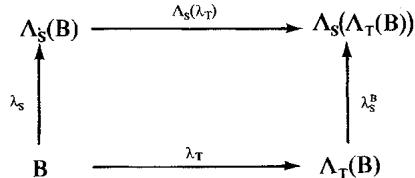
\includegraphics[keepaspectratio]{images/part001_09ec3539.jpg}}

是交换的。只需在环 B 的一个生成集上加以验证。）

\begin{enumerate}
\def\labelenumi{\alph{enumi})}
\setcounter{enumi}{1}
\tightlist
\item
  设 C 是 \(\lambda\)-环，\(\rho:A \to C\) 是 \(\lambda\)-态射，\((c_i)_{i\in I}\) 是 C 中元素的一个族。存在唯一的 \(\lambda\)-态射 \(\rho':B \to C\)，它扩张 \(\rho\)，且满足 \(\rho'(X_i) = c_i\)（对所有 \(i\in I\)）。
\end{enumerate}

\begin{enumerate}
\def\labelenumi{\arabic{enumi})}
\setcounter{enumi}{51}
\tightlist
\item
  设 \((\mathbf{A}_i)_{i\in I}\) 是一族环，\(\mathbf{A} = \prod_i\mathbf{A}_i\)，且 \(p_i:\mathbf{A}\to \mathbf{A}_i\)（对每个 \(i\in \mathbf{I}\)）是典范投影。\\
\end{enumerate}

\begin{enumerate}
\def\labelenumi{\alph{enumi})}
\item
  映射 \(\alpha :\mathbf{A}[[T]]\to \prod_i\mathbf{A}_i[[T]]\) 把 \(\sum a_n\mathbf{T}^n\) 映为 \((\sum_{n}p_i(a_n)\mathbf{T}^n)_{i\in I}\)，它是环同构。由限制，它给出环同构 \(\alpha :\Lambda (\mathbf{A})\to \prod_i\Lambda (\mathbf{A}_i)\)。此外，对所有 \(n\in \mathbf{J}\)，有 \(\alpha \circ \lambda_n^{\mathbf{A}} = (\prod_i\lambda_n^{\mathbf{A}_i})\circ \alpha\)（利用第 59 页习题 46 d) 中的“泛多项式”。）
\item
  设对每个 \(i \in I\)，\(A_i\) 都带有由 \(\lambda_i: A_i \to \Lambda(A_i)\) 给出的准\(\lambda\)-环结构。把 \(\Lambda(A)\) 与 \(\prod_{i} \Lambda(A_i)\) 通过 \(\alpha\) 等同起来，我们定义 \(\lambda = \prod_{i} \lambda_i: A \to \Lambda(A)\)。于是 \((A, \lambda)\) 是准\(\lambda\)-环，称为族 \(((A_i, \lambda_i))_{i \in I}\) 的积。\((A, \lambda)\) 是 \(\lambda\)-环当且仅当 \((A_i, \lambda_i)\) 对每个 \(i \in I\) 都是。
\end{enumerate}

\begin{enumerate}
\def\labelenumi{\arabic{enumi})}
\setcounter{enumi}{52}
\tightlist
\item
  设 \(u = 1 + \mathrm{T} + \sum_{n=2}^{\infty} a_n \mathrm{T}^n\) 是 \(\Lambda(\mathbf{Z})\) 的一个元素。存在唯一的群同态 \(\lambda^u: \mathbf{Z} \to \Lambda(\mathbf{Z})\)，使得 \(\lambda^u(1) = u\)，且 \((\mathbf{Z}, \lambda^u)\) 是准\(\lambda\)-环。有 \(\lambda^u(n) = u^n\)（对所有 \(n \in \mathbf{Z}\)）。\((\mathbf{Z}, \lambda^u)\) 是 \(\lambda\)-环当且仅当 \(u = 1 + \mathrm{T}\)，此时我们有
\end{enumerate}

\[
\lambda_ {m} ^ {1 + \mathrm{T}} (n) = \binom {n} {m} = \frac {n (n - 1) \dots (n - m + 1)}{m !}
\]

其中 \(n \in Z\)，\(m \in N\) 任意。

\begin{enumerate}
\def\labelenumi{\arabic{enumi})}
\setcounter{enumi}{53}
\tightlist
\item
  设 C 是环，A 是一个 C-代数（不必交换）。我们用 \(\mathrm{Rep}_{\mathrm{C}}(\mathbf{A})\) 表示由作为有限生成投射 C-模的 A-模的类所成的加法集，并用 \(\bar{\mathrm{R}}_{\mathrm{C}}(\mathring{\mathrm{A}})\) 表示 Grothendieck 群 K( \(\mathrm{Rep}_{\mathrm{C}}(\mathbf{A})\) )（参见 A, VIII, § 10, n° 6）。a) 设 \(\alpha : \mathrm{A}' \to \mathrm{A}\) 是 C-代数的同态。若 E 是 \(\mathrm{Rep}_{\mathrm{C}}(\mathbf{A})\) 型的 A-模，则模 \(\alpha_{*}\mathrm{E}\)（由 A 到 \(\mathrm{A}'\) 的纯量限制得到，A, II, 第 30 页）是 \(\mathrm{Rep}_{\mathrm{C}}(\mathrm{A}')\) 型的 A'-模，且 {[}E{]} \(\mapsto [\alpha_{*}\mathrm{E}]\) 定义了同态 \(\alpha_{*}: \mathrm{R}_{\mathrm{C}}(\mathrm{A}) \to \mathrm{R}_{\mathrm{C}}(\mathrm{A}')\)。
\end{enumerate}

若 \(\alpha_{1}:\mathbf{A}_{1}\to\mathbf{A}^{\prime}\) 是 C-代数的同态，则有 \((\alpha\circ\alpha_{1})_{*}=\alpha_{1*}\circ\alpha_{*}\)。

\begin{enumerate}
\def\labelenumi{\alph{enumi})}
\setcounter{enumi}{1}
\item
  令 \(\mathbf{K}_0(\mathbf{C}) = \mathbf{R}_{\mathbf{C}}(\mathbf{C})\)。结构同态 \(\varepsilon: \mathbf{C} \to \mathbf{A}\) 定义了同态 \(\varepsilon_*: \mathbf{R}_{\mathbf{C}}(\mathbf{A}) \to \mathbf{K}_0(\mathbf{C})\)。若存在 C-代数的同态 \(\gamma: \mathbf{A} \to \mathbf{C}\)，则 \(\gamma_*: \mathbf{K}_0(\mathbf{C}) \to \mathbf{R}_{\mathbf{C}}(\mathbf{A})\) 是 \(\varepsilon_*\) 的右逆。
\item
  设 \(\gamma: \mathrm{C} \to \mathrm{C}'\) 是环同态。若 E 是 \(\operatorname{Rep}_{\mathrm{C}}(\mathrm{A})\) 型的 A-模，则 \(\gamma^{*}\mathrm{E} = \mathrm{C}' \otimes_{\mathrm{C}} \mathrm{E}\) 是 \(\mathrm{A}_{\mathrm{C}'}\)-模，且是 \(\operatorname{Rep}_{\mathrm{C}'}(\mathrm{A}_{\mathrm{C}'})\) 型的，其中 \(\mathrm{A}_{\mathrm{C}'} = \mathrm{C}' \otimes_{\mathrm{C}} \mathrm{A}\)，且 {[}E{]} \(\mapsto [\gamma^{*}\mathrm{E}]\) 定义了同态 \(\gamma^{*}: \mathrm{R}_{\mathrm{C}}(\mathrm{A}) \to \mathrm{R}_{\mathrm{C}'}(\mathrm{A}_{\mathrm{C}'})\)。若 \(\gamma_{1}': \mathrm{C}' \to \mathrm{C}_{1}\) 是另一个环同态，则有 \((\gamma_{1} \circ \gamma)^{*} = \gamma_{1}^{*} \circ \gamma^{*}\)。
\item
  设 E \(\xrightarrow{f}\) F \(\xrightarrow{g}\) G 是 A-模的同态，令 \(h = g \circ f\)。构造 A-模的一个正合列
\end{enumerate}

\[
(*) \quad 0 \rightarrow \operatorname{Ker} (f) \rightarrow \operatorname{Ker} (h) \rightarrow \operatorname{Ker} (g) \rightarrow \operatorname{Coker} (f) \rightarrow \operatorname{Coker} (h) \rightarrow \operatorname{Coker} (g) \rightarrow 0.
\]

由此推出：若 \(f\) 与 \(g\) 都是单射，且 \(\operatorname{Coker}(f)\) 与 \(\operatorname{Coker}(g)\) 都是 \(\operatorname{Rep}_{\mathbb{C}}(\mathbf{A})\) 型的，则 \(\operatorname{Coker}(h)\) 是 \(\operatorname{Rep}_{\mathbb{C}}(\mathbf{A})\) 型的，并且我们有

\[
[ \operatorname{Coker} (h) ] = [ \operatorname{Coker} (f) ] + [ \operatorname{Coker} (g) ]
\]

在 \(R_{C}(A)\) 中。

\begin{enumerate}
\def\labelenumi{\arabic{enumi})}
\setcounter{enumi}{54}
\tightlist
\item
  设 C 是环。设 G 是幺半群，\(\mathbf{C}^{(\mathbf{G})}\) 是它在 C 上的代数。我们把 \(\mathrm{Rep}_{\mathbf{C}}(\mathbf{C}^{(\mathbf{G})})\) 与 \(\mathbf{R}_{\mathbf{C}}(\mathbf{C}^{(\mathbf{G})})\) 简记为 \(\mathrm{Rep}_{\mathbf{C}}(\mathbf{G})\) 与 \(\mathbf{R}_{\mathbf{C}}(\mathbf{G})\)。若 \(\alpha : \mathbf{G}' \to \mathbf{G}\) 是幺半群同态，我们也用 \(\alpha\) 表示由它定义的 C-代数同态 \(\mathbf{C}^{(\mathbf{G}')} \to \mathbf{C}^{(\mathbf{G})}\)，并用 \(\alpha_{*}: \mathbf{R}_{\mathbf{C}}(\mathbf{G}) \to \mathbf{R}_{\mathbf{C}}(\mathbf{G}')\) 表示相应的同态。
\end{enumerate}

根据 A, VIII, § 10, n° 5，在 R \(_{C}\) (G) 上存在一个（交换）环结构，使得

\[
[ \mathbf {E} ]. [ \mathbf {F} ] = [ \mathbf {E} \otimes_ {\mathrm{C}} \mathbf {F} ]
\]

其中 E 与 F 是 \(\mathrm{Rep}_{\mathbb{C}}(\mathbf{G})\) 型的有限型模。这个乘法的单位元是模 \(C_1\) 的类，即带有 G 的平凡作用的 C。

\begin{enumerate}
\def\labelenumi{\alph{enumi})}
\tightlist
\item
  环 \(\mathbf{R}_{\mathrm{C}}(\mathbf{G})\) 具有唯一的准-\(\lambda\)-环结构，使得
\end{enumerate}

\[
\lambda [ \mathrm{E} ] = \sum_ {n \geqslant 0} \left[ \Lambda ^ {n} (\mathrm{E}) \right] \mathbf {T} ^ {n}
\]

对每个 \(\mathrm{Rep}_{\mathrm{C}}(\mathrm{G})\) 型的有限型模 E 成立。（首先注意 \(\Lambda^{\mathrm{n}}(\mathrm{E})\) 仍是 \(\mathrm{Rep}_{\mathrm{C}}(\mathrm{G})\) 型的有限型模。然后，设 F 是使 F 与 E/F 都是 \(\mathrm{Rep}_{\mathrm{C}}(\mathrm{G})\) 型有限型模的子模，证明

\[
\left[ \Lambda ^ {n} (\mathrm{E}) \right] = \sum_ {p = 0} ^ {n} \left[ \Lambda ^ {p} (\mathrm{F}) \otimes_ {\mathrm{C}} \Lambda ^ {n - p} (\mathrm{E/F}) \right].
\]

在 \(\mathbf{R}_{\mathbf{C}}(\mathbf{G})\) 中成立。）为此，用 \(\mathbf{L}_p\) 表示 \(\Lambda^p(\mathbf{F}) \otimes_{\mathbf{C}} \Lambda^{n-p}(\mathbf{E})\) 在乘法之下在 \(\Lambda^n(\mathbf{E})\) 中的像。我们有 \(\Lambda^n(\mathbf{E}) = \mathbf{L}_0 \supset \mathbf{L}_1 \supset \ldots \supset \mathbf{L}_n = \Lambda^n(\mathbf{F}) \supset \mathbf{L}_{n+1} = 0\)，并且存在 \(\mathbf{C}^{(\mathbf{G})}\)-模的典范同构，把 \(\mathbf{L}_p / \mathbf{L}_{p+1}\) 映到 \(\Lambda^p(\mathbf{F}) \otimes \Lambda^{n-p}(\mathbf{E}/\mathbf{F})\) 上。

\begin{enumerate}
\def\labelenumi{\alph{enumi})}
\setcounter{enumi}{1}
\item
  对每个幺半群同态 \(\alpha: \mathbf{G}' \to \mathbf{G}\)，映射 \(\alpha_*: \mathbf{R}_{\mathbf{C}}(\mathbf{G}) \to \mathbf{R}_{\mathbf{C}}(\mathbf{G}')\) 是 \(\lambda\)-态射。特别地，\(\mathbf{K}_0(\mathbf{C})\) 是准-\(\lambda\)-环，且 \(\varepsilon_*: \mathbf{R}_{\mathbf{C}}(\mathbf{G}) \to \mathbf{K}_0(\mathbf{C})\) 是 \(\lambda\)-态射。同态 \(\mathbf{G} \to \{1\}\) 给出它的一个右逆。
\item
  设 \(\mathbf{G}\) 是幺半群，\(\mathbf{R}\) 是一个集合。若函数 \(f: \mathbf{G} \to \mathbf{R}\) 满足 \(f(st) = f(ts)\)（对任意 \(s, t \in \mathbf{G}\)），则称它为中心函数。用 FC(G, R) 表示这些函数所成的集合。若 R 是 \(\lambda\)-环，则 FC(G, R) 典范地带有 \(\lambda\)-环的结构，使得
\end{enumerate}

\[
\begin{array}{r l} (f + f ^ {\prime}) (s) & = f (s) + f ^ {\prime} (s) \\ (f \cdot f ^ {\prime}) (s) & = f (s) \cdot f ^ {\prime} (s) \\ (\lambda_ {n} f) (s) & = \lambda_ {n} (f (s)) \end{array}
\]

其中 \(f, f'\) 是 \(\mathrm{FC}(\mathbf{G}, \mathbf{R})\) 中的任意元素，\(s\) 属于 \(\mathbf{G}\)。这一构造特别适用于 \(\mathbf{R} = \Lambda(\mathbf{C})\) 的情形。

\begin{enumerate}
\def\labelenumi{\alph{enumi})}
\setcounter{enumi}{3}
\tightlist
\item
  设 E 是 \(\mathrm{Rep}_{\mathbb{C}}(\mathbf{G})\) 型的有限型模。对每个 \(s \in \mathbf{G}\)，用 \(s_{\mathbb{E}}\) 表示 E 中比为 \(s\) 的位似，并令
\end{enumerate}

\[
\overline {{{{\chi}}}} _ {\mathrm{E}} (s) = \det _ {\mathrm{E} [ \mathrm{T} ]} (1 + s _ {\mathrm{E}} \mathrm{T}) \in \Lambda (\mathrm{C})
\]

（参见第 62 页习题 49）。证明

\[
\overline {{{{\chi}}}}: [ \mathrm{E} ] \mapsto \overline {{{{\chi}}}} _ {\mathrm{E}}
\]

定义了一个 λ-态射

\[
\overline {{{{\chi}}}}: \mathrm{R} _ {\mathrm{C}} (\mathrm{G}) \rightarrow \mathrm{FC} (\mathrm{G}, \Lambda (\mathrm{C})).
\]

\begin{enumerate}
\def\labelenumi{\alph{enumi})}
\setcounter{enumi}{4}
\tightlist
\item
  若 C 是域，则 \(\overline{\chi}\) 是单射（A, VIII, § 10, n° 6，命题 10）。试在此情形推出 \(R_{C}(G)\) 是 \(\lambda\)-环。
\end{enumerate}

\begin{enumerate}
\def\labelenumi{\arabic{enumi})}
\setcounter{enumi}{55}
\tightlist
\item
  设 G 是由一个元素 T 生成的自由幺半群，于是 \(\mathrm{C}^{(\mathrm{G})}\) 等同于 C{[}T{]}。用 \(C_{0}\) 表示模 \(C{[}T{]}/T C{[}T{]}\)。则 \([C_{0}]\) 是 \(\mathrm{R}_{\mathrm{C}}(\mathrm{C}[\mathrm{T}])\) 的一个幂等元。典范 \(\lambda\)-态射 \(\mathrm{R}_{\mathrm{C}}(\mathrm{C}[\mathrm{T}]) \rightarrow \mathrm{K}_{0}(\mathrm{C})\) 的核是由 \(1 - [\mathrm{C}_{0}]\) 生成的理想。令
\end{enumerate}

\[
\tilde {\mathrm{R}} _ {\mathrm{C}} (\mathrm{C} [ \mathrm{T} ]) = \mathrm{R} _ {\mathrm{C}} (\mathrm{C} [ \mathrm{T} ]) / [ \mathrm{C} _ {0} ]. \mathrm{R} _ {\mathrm{C}} (\mathrm{C} [ \mathrm{T} ]).
\]

\begin{enumerate}
\def\labelenumi{\alph{enumi})}
\item
  证明 \([C_{0}].R_{C}(C[T])\) 是 \(\lambda\)-理想，从而 \(\tilde{R}_{C}(C[T])\) 具有一个商准-\(\lambda\)-环。
\item
  对每个 \(\operatorname{Rep}_{\mathbf{C}}(\mathbf{C}[\mathbf{T}])\) 型的有限型模 E，用 \(\mathbf{T}_{\mathbf{E}}\) 表示 E 中比为 T 的位似。我们有
\end{enumerate}

以及

\[
\begin{array}{l} \overline {{\chi}} _ {\mathrm{E}} (\mathrm{T}) = \det _ {\mathrm{E} [ \mathrm{T} ]} (1 + \mathrm{T} _ {\mathrm{E}} \mathrm{T}) \in \Lambda (\mathrm{C}) \\ \chi_ {\mathrm{E}} (\mathrm{T}) = \det _ {\mathrm{E} [ \mathrm{T} ]} (\mathrm{T} - \mathrm{T} _ {\mathrm{E}}) \end{array}
\]

是 \(T_{E}\) 的特征多项式（参见第 62 页习题 49）。证明 \([E] \mapsto \overline{\chi}_{E}(T)\) 定义了一个 \(\lambda\)-态射 \(R_{C}(C[T]) \to \Lambda(C)\)，它的核包含 \([C_{0}]\)。通过过渡到商，我们得到 \(\lambda\)-态射

\[
\overline {{\chi}}: \tilde {\mathrm{R}} _ {\mathrm{C}} (\mathrm{C} [ \mathrm{T} ]) \to \Lambda (\mathrm{C}).
\]

\begin{enumerate}
\def\labelenumi{\alph{enumi})}
\setcounter{enumi}{2}
\item
  用 \(\Lambda_{\mathrm{rat}}(\mathbf{C})\) 表示 \(\Lambda(\mathbf{C})\) 的由 \(\Lambda(\mathbf{C})\) 中 T 的多项式元素所生成的子群。证明 \(\overline{\chi}\) 的像是 \(\Lambda_{\mathrm{rat}}(\mathbf{C})\)。由此得出 \(\Lambda_{\mathrm{rat}}(\mathbf{C})\) 是一个子 \(\lambda\)-环，包含在 \(\Lambda(\mathbf{C})\) 中。
\item
  对每个 \(r \in \mathbf{Z}\)，定义 \(\sigma_r: \mathrm{C}[\mathrm{T}, \mathrm{T}^{-1}] \to \mathrm{C}[\mathrm{T}, \mathrm{T}^{-1}]\) 为 \((\sigma_r f)(\mathrm{T}) = \mathrm{T}^{r} f((-\mathrm{T})^{-1})\)。我们有 \((\sigma_r(\sigma_s f))(\mathrm{T}) = (-1)^s \mathrm{T}^{r-s} f(\mathrm{T})\)，特别地 \(\sigma_r(\sigma_r f) = (-1)^r f\)，以及 \((\sigma_r f).(\sigma_s g) = \sigma_{r+s}(f.g)\)（\(r, s\) 取遍 \(\mathbf{Z}\)，\(f, g\) 取遍 \(\mathrm{C}[\mathrm{T}, \mathrm{T}^{-1}]\)）。若 \(f\) 是 \(T\) 的次数 \(\leqslant r\)（\(r \geqslant 0\)）的多项式，则 \(\sigma_r f\) 也是。此外，若 \(f \in \Lambda(\mathrm{C})\)（即 \(f(0) = 1\)），则 \(\sigma_r f\) 是次数为 \(r\) 的首一多项式。若 E 是 C{[}T{]}-模，且是秩为 \(r\) 的自由 C-模，则有 \(\sigma_r(\overline{\chi}_{\mathrm{E}}(\mathrm{T})) = \chi_{\mathrm{E}}(\mathrm{T})\)。e) 若 \(f \in \Lambda(\mathrm{C})\) 是 \(T\) 的次数 \(\leqslant r\) 的多项式，令 \(E_{r,f} = C[T]/\sigma_r f.C[T]\)；它是秩为 \(r\) 的自由 C-模。若 \(f = 1\)，我们有 \(E_{r,1} = C[T]/T^{r}C[T]\)。若 \(g \in \Lambda(\mathrm{C})\) 是 \(T\) 的次数 \(\leqslant s\) 的多项式，则有 C{[}T{]}-模的一个正合列
\end{enumerate}

\[
(*) \quad 0 \rightarrow \mathrm{E} _ {s, g} \rightarrow \mathrm{E} _ {r + s, f g} \rightarrow \mathrm{E} _ {r, f} \rightarrow 0
\]

（利用 \(d\)）。）证明 \(\tau(f)\)（\(\mathrm{E}_{r,f}\) 在 \(\tilde{\mathrm{R}}_{\mathrm{C}}(\mathrm{C}[\mathrm{T}])\) 中的类）与 \(r\)（ \(\geqslant \deg(f)\) ）无关。（事实上，\(\sigma_{r+s}f = (\sigma_s1).(\sigma_rf) = \mathrm{T}^s.(\sigma_rf)\)，而模 \(\mathrm{C}[\mathrm{T}] / \mathrm{T}^s\mathrm{C}[\mathrm{T}]\) 在 \(\tilde{\mathrm{R}}_{\mathrm{C}}(\mathrm{C}[\mathrm{T}])\) 中的类为零。）证明：若 \(g\) 是 \(\Lambda(\mathrm{C})\) 中的多项式，则有 \(\tau(fg) = \tau(f) + \tau(g)\)。（再次利用正合列 (*)。）由此推出，\(\tau\) 可扩张为群同态

\[
\tau : \Lambda_ {\mathrm{rat}} (\mathrm{C}) \rightarrow \tilde {\mathrm{R}} _ {\mathrm{C}} (\mathrm{C} [ \mathrm{T} ]).
\]

\begin{enumerate}
\def\labelenumi{\alph{enumi})}
\setcounter{enumi}{5}
\tightlist
\item
  证明 \(\overline{\chi} \circ \tau\) 是 \(\Lambda_{\mathrm{rat}}(\mathbf{C})\) 的恒等映射（利用下述事实：若 \(f \in \Lambda(\mathbf{C})\) 是次数 \(\leqslant r\) 的多项式，则 \(\mathrm{T}_{\mathrm{E}_r,f}\) 的特征多项式是 \(\sigma_r f\)。）
\item
  证明 \(\tilde{\mathrm{R}}_{\mathrm{C}}(\mathrm{C}[\mathrm{T}])\) 的每个元素都是某个作为自由 C-模的 C{[}T{]}-模 E 的类。
\end{enumerate}

\(h\) ) 设 E 是 C{[}T{]}-模，用 \(u\in \mathrm{End}_{\mathrm{C}}(\mathrm{E})\) 表示 E 中比为 T 的位似；令 \(\overline{u} = \mathrm{Id}_{\mathrm{C[T]}}\otimes_{\mathrm{C}}u\in \mathrm{End}_{\mathrm{C[T]}}(\mathrm{E}[\mathrm{T}])\)。我们有一个 C{[}T{]}-模的正合列

\[
0 \longrightarrow \mathrm{E} [ \mathrm{T} ] \xrightarrow {\mathrm{T} - \bar {u}} \mathrm{E} [ \mathrm{T} ] \longrightarrow \mathrm{E} \longrightarrow 0
\]

（A, III, 第 106 页）。设 E 是以 \((e_1, \ldots, e_r)\) 为基的自由 C-模。则 E{[}T{]} 是自由 C{[}T{]}-模，以 \((1 \otimes e_i)\) 为基。若 \(u\) 在基 \((e_i)\) 下的矩阵是 \((a_{ij})\)，则 T - \(\overline{u}\) 在基 \((1 \otimes e_i)\) 下的矩阵是 \((\mathrm{T}\delta_{ij} - a_{ij})\)。

\begin{enumerate}
\def\labelenumi{\roman{enumi})}
\tightlist
\item
  设 \(f = (f_{ij})_{1 \leqslant i,j \leqslant r}\) 是系数在 C{[}T{]} 中的矩阵。则称 \(f\) 为特殊矩阵，如果对所有 \(i, j\)（属于 \(\{1, \dots, r\}\) 且 \(i \neq j\)），\(f_{ii}\) 都是首一多项式且 \(\deg(f_{ii}) > \deg(f_{ij})\)。证明 \(\det(f)\) 是首一多项式（次数为 \(\deg(f_{11}) + \cdots + \deg(f_{rr})\)），且 \(f\) 定义了 C{[}T{]} \(^r\) 的一个单射自同态。由 h) 推出：每个 C{[}T{]}-模，只要是秩为 \(r\) 的自由 C-模，就同构于 C{[}T{]} \(^r\) 的这样一个自同态的余核。
\end{enumerate}

\begin{enumerate}
\def\labelenumi{\alph{enumi})}
\setcounter{enumi}{9}
\tightlist
\item
  设 f 是如 i) 中的特殊矩阵。置 \(f = \begin{pmatrix} f_{11} & f_{+} \\ f_{-} & f' \end{pmatrix}\)，其中 \(f_{+}\)，\(f_{-}\)，\(f'\) 分别是 \((1, r - 1)\)，\((r - 1, 1)\) 与 \((r - 1, r - 1)\) 型的矩阵。令
\end{enumerate}

\[
g = \left( \begin{array}{c c} 1 & 0 \\ - f _ {-} & f _ {1 1} \mathrm{I} \end{array} \right) \quad \text {and} \quad h = g f = \left( \begin{array}{c c} f _ {1 1} & f _ {+} \\ 0 & \overline {{f}} \end{array} \right) \quad \text {where} \quad \overline {{f}} = f _ {1 1} f ^ {\prime} - f _ {-} f _ {+}.
\]

证明 h 是特殊矩阵。此外，把方阵与相应的自同态等同起来，就得到 C{[}T{]}-模的正合列

\[
0 \rightarrow \operatorname{Coker} (f) \rightarrow \operatorname{Coker} (h) \rightarrow \operatorname{Coker} (g) \rightarrow 0,
\]

（其中 Coker(g) 同构于 \(\mathbf{C}[\mathbf{T}]^{r - 1} / f_{11}\mathbf{C}[\mathbf{T}]^{r - 1}\) ）以及

\[
0 \rightarrow \mathrm{C} [ \mathrm{T} ] / f _ {1 1} \mathrm{C} [ \mathrm{T} ] \rightarrow \operatorname{Coker} (h) \rightarrow \operatorname{Coker} (\bar {f}) \rightarrow 0.
\]

由此对 \(r\) 作归纳推出：\(\operatorname{Coker}(f)\) 是投射 C-模，且它在 \(\mathbf{R}_{\mathrm{C}}(\mathbf{C}[\mathrm{T}])\) 中的类是 \(\mathbf{Z}\)-线性组合，其项形如 \([\mathbf{C}[\mathrm{T}] / p\mathbf{C}[\mathrm{T}]]\)，其中 \(p\) 是首一多项式。

  \(k\) ) 利用前面的 \(f\)、\(g\)、\(i)\) 与 \(j)\) 各款，证明 \(\tau : \Lambda_{\mathrm{rat}}(\mathbf{C}) \to \tilde{\mathbf{R}}_{\mathrm{C}}(\mathbf{C}[\mathrm{T}])\) 是满射，从而 \(\overline{\chi} : \tilde{\mathbf{R}}_{\mathrm{C}}(\mathbf{C}[\mathrm{T}]) \to \Lambda_{\mathrm{rat}}(\mathbf{C})\) 是同构。

\begin{enumerate}
\def\labelenumi{\alph{enumi})}
\setcounter{enumi}{11}
\tightlist
\item
  证明 \(\Lambda_{\mathrm{rat}}(\mathbf{C})\) 在 \(\mathbf{V}_n\) 与 \(\mathbf{F}_n\) 之下稳定（对每个 \(n \in \mathbf{J}\)）。于是它们借助上述同构对应于 \(\mathbf{V}_n\) 与 \(\mathbf{F}_n\)，即 \(\tilde{\mathbf{R}}_{\mathbf{C}}(\mathbf{C}[\mathbf{T}])\) 的自同态。设 \(\varphi_n\) 是 C{[}T{]} 到其自身的、把 T 映为 \(\mathbf{T}^n\) 的 C-代数同态。证明 \(\mathbf{V}_n\)（相应地 \(\mathbf{F}_n\)）是通过过渡到商从自同态 \(\varphi_n^*\)（相应地 \((\varphi_n)_*\)）导出的，这些自同态定义在 \(\mathbf{R}_{\mathbf{C}}(\mathbf{C}[\mathbf{T}])\) 上。
\end{enumerate}

在以下各习题中，p 是一个固定的素数，且 Witt 向量环都是相对于这个素数而言的。

\begin{enumerate}
\def\labelenumi{\arabic{enumi})}
\setcounter{enumi}{56}
\tightlist
\item
  设 \(m\), \(n\) 是两个 \(\geqslant 1\) 的整数。对每个特征为 \(p\) 的环 A，用 \(_{m}\mathrm{W}_{n}(\mathrm{A})\) 表示 \(\mathrm{F}^{m}\)（\(\mathrm{W}_{n}(\mathrm{A})\) 的自同态）的核。
\end{enumerate}

\begin{enumerate}
\def\labelenumi{\alph{enumi})}
\tightlist
\item
  当 \(m \geqslant 2\) 且 \(n \geqslant 1\) 时，下图是交换的
\end{enumerate}

\pandocbounded{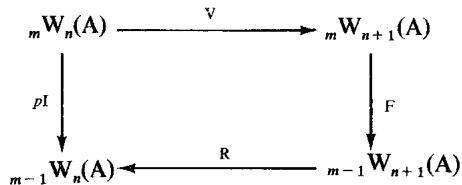
\includegraphics[keepaspectratio]{images/part001_6a9997c3.jpg}}

其中映射 V，F 分别由位移同态与 Frobenius 同态诱导，I 是自然单射，R 是自然投影。

\begin{enumerate}
\def\labelenumi{\alph{enumi})}
\setcounter{enumi}{1}
\tightlist
\item
  对 \(n \geqslant 1\) 以及 \(a = [a_0, \ldots, a_{n-1}]\)（属于 \(W_n(A)\)），用 \(\tilde{a}\) 表示 \((a_0, \ldots, a_{n-1}, 0, \ldots)\)，即 \(W(A)\) 的元素。
\end{enumerate}

设 \(a \in_{m} W_{n}(A)\)，\(b \in_{n} W_{m}(A)\)。令

\[
\langle \boldsymbol {a}, \boldsymbol {b} \rangle = \mathrm{E} (\omega_ {\mathrm{A}} (\tilde {\boldsymbol {a}}) \omega_ {\mathrm{A}} (\tilde {\boldsymbol {b}}), 1)
\]

（记号 E 参见第 57 页习题 43，记号 \(\omega_{\mathbf{A}}\) 参见第 54 页习题 40。）证明映射 \((\boldsymbol{a}, \boldsymbol{b}) \mapsto \langle \boldsymbol{a}, \boldsymbol{b} \rangle\)（从 \({}_{m}W_n(A) \times {}_{n}W_m(A)\) 到 \(A^*\)）是 \(\mathbf{Z}\)-双线性的。c) 采用 a) 中的记号，我们有

\[
\langle \boldsymbol {a}, \mathrm{V} \boldsymbol {b} \rangle = \langle \mathrm{F} \boldsymbol {a}, \boldsymbol {b} \rangle . \text { for } \quad \boldsymbol {a} \in_ {m} \mathrm{W} _ {n} (\mathrm{A}) \quad \text { and } \quad \boldsymbol {b} \in_ {n} \mathrm{W} _ {m - 1} (\mathrm{A})
\]

以及

\[
\langle \mathbf {R} \boldsymbol {a}, \boldsymbol {b} \rangle = \langle \boldsymbol {a}, \mathbf {I} \boldsymbol {b} \rangle \quad \text { for } \quad \boldsymbol {a} \in_ {m} \mathrm{W} _ {n} (\mathrm{A}) \quad \text { and } \quad \boldsymbol {b} \in_ {n - 1} \mathrm{W} _ {m} (\mathrm{A}).
\]

\begin{enumerate}
\def\labelenumi{\arabic{enumi})}
\setcounter{enumi}{57}
\tightlist
\item
  \begin{enumerate}
  \def\labelenumii{\alph{enumii})}
  \tightlist
  \item
    设 \(\delta(T)\) 是形式级数 \(\exp\left(-\sum_{n=0}^{\infty}\mathrm{T}^{p^n}/p^n\right)\)（\(\mathbf{Q}[[T]]\) 中的）。我们有
  \end{enumerate}
\end{enumerate}

\[
\mathfrak{E}(\mathrm{T}) = \prod_{\substack{(n,p) = 1\\ n\text{ 为整数}\geqslant 1}}(1 - \mathrm{T}^{n})^{\mu (n) / n}
\]

其中 μ 是 Möbius 函数。δ(T) 的系数都属于 \(\mathbf{Z}_{(p)}\)。b) 设 \(\mathbf{X} = (\mathbf{X}_{n})_{n \in \mathbb{N}}\) 是一族未定元。在代数 \(\mathbf{Q}[(\mathbf{X}_{n})_{n \in \mathbb{N}}]\) 中，我们有等式

\[
\prod_ {n = 0} ^ {\infty} \mathcal {E} (\mathrm{X} _ {n} \mathrm{T} ^ {p ^ {n}}) = \exp \left(- \sum_ {n = 0} ^ {\infty} \Phi_ {n} (\mathrm{X}) \mathrm{T} ^ {p ^ {n}} / p ^ {n}\right).
\]

\begin{enumerate}
\def\labelenumi{\alph{enumi})}
\setcounter{enumi}{2}
\item
  设 A 是 \(\mathbf{Z}_{(p)}\) -代数。假设 A 中乘以 \(p, 1_{\mathbf{A}}\) 的乘法是单射。设 \(\boldsymbol{a} = (a_n)_{n \in \mathbb{N}} \in \mathbb{A}^{\mathbf{N}}\)。级数 \(\exp\left(\sum_{n=0}^{\infty} a_n \mathbf{T}^{p^n} / p^n\right)\)（\(\mathrm{A}\left[\frac{1}{p}\right]\) {[}{[}T{]}{]} 中的）的系数都属于 A，当且仅当 \(\boldsymbol{a}\) 属于 \(\Phi_{\Lambda}(\mathbf{W}(\mathbf{A}))\)。
\item
  设 A 是 \(\mathbf{Z}_{(p)}\)-代数。映射 \(\mathbf{E} \circ \omega_{\Lambda}\)（从 W(A) 到 \(\Lambda(\mathbf{A})\)，参见第 54 页习题 40 及第 57 页习题 43）把 \(\boldsymbol{a} = (a_n)_{n \in \mathbb{N}}\) 映为 \(\prod_{n=0}^{\infty} \delta(a_n(-\mathbf{T})^{p^n})\)（\(\Lambda(\mathbf{A})\) 的元素）。
\item
  设 A 是 \(\mathbf{Z}_{(p)}\)-代数。假设 A 中乘以 \(p,1_{A}\) 的乘法是单射。设 \(\sigma\) 是 A 的满足 \(\sigma a \equiv a^{p} \mod pA\) 的自同态。设 \(s_{\sigma}:A \to W(A)\) 是与 \(\sigma\) 相伴的同态（第 44 页习题 14）。于是，对每个 \(a \in A\)，形式级数
\end{enumerate}

\[
\mathrm{E} _ {\sigma} (a, \mathrm{T}) = \exp (\sum_ {i = 0} ^ {\infty} \sigma^ {i} (a) \mathrm{T} ^ {p ^ {i}} / p ^ {i})
\]

的系数都属于 A，并且我们有

\[
\mathrm{E} \circ \omega_ {\mathrm{A}} \circ s _ {\sigma} (a ^ {- 1}) = \exp \left(\sum_ {i = 0} ^ {\infty} \sigma^ {i} (a) (- \mathrm{T}) ^ {p ^ {i}} / p ^ {i}\right) = \mathrm{E} _ {\sigma} (a, - \mathrm{T}).
\]

\begin{enumerate}
\def\labelenumi{\alph{enumi})}
\setcounter{enumi}{5}
\tightlist
\item
  设 \(\mathcal{A}\) 是环 \(\mathbf{Z}_{(p)}[(\mathbf{X}_n)_{n\in\mathbb{N}}]\)，且 \(\mathbf{X} = (\mathbf{X}_n)_{n\in\mathbb{N}} \in \mathrm{W}(\mathcal{A})\)。级数 \(\mathrm{E}_{\mathrm{F},\mathcal{A}}(\mathbf{X},\mathrm{T})\) 的系数都属于 \(\mathrm{W}(\mathcal{A})\)。对每个 \(\mathbf{Z}_{(p)}\) -代数 A 以及 \(a = (a_n)_{n\in\mathbb{N}}\)（\(\mathrm{W}(\mathrm{A})\) 的元素），我们把 \(\mathrm{E}_{\mathrm{F}}(a,\mathrm{T})\) 记为通过 \(\mathrm{W}(\varphi)\) 作用于 \(\mathrm{E}_{\mathrm{F},\mathcal{A}}(\mathbf{X},\mathrm{T})\) 的系数所得到的级数，其中 \(\varphi: \mathcal{A} \to \mathrm{A}\) 是把 \(\mathrm{X}_n\) 映到 \(a_n\) 的映射。于是 \(\mathrm{E}_{\mathrm{F}}(a,\mathrm{T})\) 的系数都属于 \(\mathrm{W}(\mathrm{A})\)，且若 \(s_{\mathrm{A}}\) 表示第 44 页习题 15 中定义的同态 \(\mathrm{W}(\mathrm{A}) \to \mathrm{W}(\mathrm{W}(\mathrm{A}))\)，我们有
\end{enumerate}

\[
\mathrm{E} \circ \omega_ {\mathrm{W(A)}} \circ s _ {\mathrm{A}} (\boldsymbol {a} ^ {- 1}) = \mathrm{E} _ {\mathrm{F}} (\boldsymbol {a}, - \mathrm{T}) \quad \text { for all } \quad \boldsymbol {a} \in \mathrm{W(A)}.
\]

\exercisesection{COHEN 环}

在 § 2 的习题中，\(p\) 是一个固定的素数。若 \(a\) 是环 A 的理想，则用 \(a^p\) 表示由元素 \(a^p\)（其中 \(a\) 取遍 \(a\)）所生成的理想。

\begin{enumerate}
\def\labelenumi{\arabic{enumi})}
\item
  设 \((\mathbf{C}_{n}, \pi_{n,m})\) 是关于指标集 N 的环的逆系统。假设 \(C_{n}\)（对每个 \(n \in N\)）都是 Artin 环，且诸同态 \(\pi_{n,m}\) 都是满射。设 \(\pi_{n}\) 是从 \(C = \varprojlim C_{n}\) 到 \(C_{n}\) 的典范同态。证明对所有 \(x \in C\)，有 \(xC = \varprojlim \pi_{n}(x) C_{n}\)。（按 § 2, n° 1 命题 3 的证明方式处理。）
\item
  设 A 是环，\((\mathbf{J}_{n})_{n\in\mathbb{N}}\) 是 A 的理想的一个递降序列，使得有 \(pJ_{n} + J_{n}^{p} \subset J_{n+1}\)（对每个 \(n \in N\)）。
\end{enumerate}

\begin{enumerate}
\def\labelenumi{\alph{enumi})}
\item
  证明在这一假设下，§ 1, n° 1 的引理 1 与命题 1 的断言仍然成立。
\item
  设 \(i\) 与 \(n\) 是两个正整数。当 \(i \leqslant n\) 时，从 A 到 A 的映射 \(x \mapsto p^i x^{p^n - i}\) 通过过渡到商定义了一个映射
\end{enumerate}

\[
\rho_ {n, i} ^ {\mathbf {A}}: \mathrm{A} / \mathrm{J} _ {0} \rightarrow \mathrm{A} / \mathrm{J} _ {n}.
\]

当 \(i > n\) 时，令 \(\rho_{n,i}^{\mathbf{A}} = 0\)。对 \(x \in \mathrm{A} / \mathrm{J}_n\) 与 \(a \in \mathrm{A} / \mathrm{J}_0\)，有 \(x^{p^{n - i}} \rho_{n,i}^{\mathbf{A}}(a) = \rho_{n,i}^{\mathbf{A}}(\overline{x} a)\)，其中 \(\overline{x}\) 是 \(x\) 在 \(\mathrm{A} / \mathrm{J}_0\) 中的像。若 \(j\) 是正整数，且 \(a, b\) 是 \(\mathrm{A} / \mathrm{J}_n\) 的两个元素，则有

\[
\rho_ {n, i} ^ {\mathbf {A}} (a) \rho_ {n, j} ^ {\mathbf {A}} (b) = \rho_ {n, i + j} ^ {\mathbf {A}} \left(a ^ {p ^ {j}} b ^ {p ^ {i}}\right).
\]

\begin{enumerate}
\def\labelenumi{\alph{enumi})}
\setcounter{enumi}{2}
\tightlist
\item
  设 \((\mathbf{R}_{n})_{n\in\mathbf{N}}\) 是第 42 页习题 3 中构造的多项式序列。设 n 与 i 是两个正整数，a 与 b 是 \(A/J_{0}\) 的两个元素。于是在 \(A/J_{n}\) 中有等式
\end{enumerate}

\[
\rho_ {n, i} ^ {\mathrm{A}} (a) + \rho_ {n, i} ^ {\mathrm{A}} (b) = \sum_ {m = 0} ^ {n - i} \rho_ {n, i + m} ^ {\mathrm{A}} (\mathrm{R} _ {m} (a, b)).
\]

\begin{enumerate}
\def\labelenumi{\arabic{enumi})}
\setcounter{enumi}{2}
\tightlist
\item
  设 \(n\) 是正整数。设 C 是 \(p\)-Cohen 环，其剩余域为 \(k\)，长度为 \(n+1\)。设 \((x_{\lambda})_{\lambda\in\Lambda}\) 是 C 中提升 \(p\)-基 \((\xi_{\lambda})_{\lambda\in\Lambda}\)（\(k\) 的）的元素族。用 \(\rho_{i}:k\to C\)（对每个 \(i\in\mathbf{N}\)）表示习题 2 中定义的映射 \(\rho_{n,i}^{\mathrm{C}}\)，其中 \(\mathbf{J}_{m}\) 取理想 \(p^{m+1}\mathbf{C}\)。
\end{enumerate}

\begin{enumerate}
\def\labelenumi{\alph{enumi})}
\tightlist
\item
  对 \(r \in \mathbf{N}\)，用 \(\mathbf{M}_r\) 表示由重指标 \(m \in \mathbf{N}^{(\Lambda)}\)（满足对每个 \(\lambda \in \Lambda\) 有 \(0 \leqslant m_{\lambda} < p^{r}\)）所成的集合。于是，对 C 的每个元素 \(\alpha\)，存在唯一的有限支撑族 \((a_{i,m})\)（\(0 \leqslant i \leqslant n\)，\(m \in \mathbf{M}_{n-i}\)），其元素属于 \(k\)，使得
\end{enumerate}

\[
\alpha = \sum_ {i = 0} ^ {n} \sum_ {m \in \mathbf {M} _ {n - i}} \rho_ {i} (a _ {i, m}) x ^ {m},
\]

其中记号 \(x^{m}\) 表示乘积 \(\prod x_{\lambda}^{m_{\lambda}}\)。

\begin{enumerate}
\def\labelenumi{\alph{enumi})}
\setcounter{enumi}{1}
\tightlist
\item
  考虑由生成元 \([x_{\lambda}]\)（\(\lambda\) 取遍 \(\Lambda\)）与 \([\rho_{i}(a)]\)（i 取遍 N，a 取遍 k）所生成的环 U，这些生成元只须满足下列关系（其中多项式 \(R_{i}\) 是第 42 页习题 3 中引入的那些）。
\end{enumerate}

\begin{enumerate}
\def\labelenumi{(\roman{enumi})}
\item
  \([\rho_i(a)] = 0\) 对 \(a \in k, i > n\) 成立，
\item
  \(\left[\rho_0(1)\right] = 1\) 且 \(\left[\rho_0(0)\right] = 0,\)
\item
  \([\rho_i(a)][\rho_j(b)] = [\rho_{i + j}(a^{p^j}b^{p^i})]\) 对 \(i,j\)（属于 \(\mathbf{N}\)）与 \(a,b\)（属于 \(k\)）成立，
\item
  \([\rho_i(a)] + [\rho_i(b)] = \sum [\rho_{i+m}(\mathbf{R}_m(a,b))]\)（对 \(i\in \mathbf{N}\) 与 \(a,b\)（属于 \(k,\)）），
\item
  \([x_{\lambda}]^{p^{n - i}}[\rho_i(a)] = [\rho_i(\xi_{\lambda}a)]\) 对 \(0 \leqslant i \leqslant n, \lambda \in \Lambda, a \in k\) 成立。
\end{enumerate}

证明我们有 \([\rho_i(0)] = 0\)（对每个 \(i \in \mathbf{N}\)）。

利用第 42 页习题 3 b) 证明：若 \(p\) 为奇数，则有 \([\rho_0(-1)] = -1\)；若 \(p\) 为偶数，则有 \(\sum_{i=0}^{n} [\rho_i(1)] = -1\)。

\begin{enumerate}
\def\labelenumi{\alph{enumi})}
\setcounter{enumi}{2}
\tightlist
\item
  存在唯一的从 U 到 C 的映射，它把 U 中与每个有限支撑族 \((a_{i,m})_{0\leqslant i\leqslant n,m\in M_{n - i}}\)（其元素属于 \(k\)）相伴的元素
\end{enumerate}

\[
\left\langle \left(a _ {i, m}\right) \right\rangle = \sum_ {i = 0} ^ {n} \sum_ {m \in \mathbf {M} _ {n - i}} \left[ \rho_ {i} (a _ {i, m}) \right] \prod_ {\lambda \in \Lambda} [ x _ {\lambda} ] ^ {m _ {\lambda}}
\]

映到 C 的元素 \(\sum_{i=0}^{n}\sum_{m\in M_{n-i}}\rho_i(a_{i,m})x^m\)；它是环同构。

\begin{enumerate}
\def\labelenumi{\alph{enumi})}
\setcounter{enumi}{3}
\tightlist
\item
  由前述结果给出 § 2, n° 3 各结果的另一个证明。
\end{enumerate}

\begin{enumerate}
\def\labelenumi{\arabic{enumi})}
\setcounter{enumi}{3}
\tightlist
\item
  设 C 是无限长度的 \(p\)-Cohen 环，\(k\) 是其剩余域。设 A 是环，\((\mathbf{J}_n)_{n \in \mathbb{N}}\) 是 A 的理想的递降序列，满足 \(p\mathbf{J}_n + \mathbf{J}_n^p \subset \mathbf{J}_{n+1}\)（对每个 \(n \in \mathbb{N}\)）。最后，设 \(\overline{\varphi}: k \to \mathrm{A} / \mathrm{J}_0\) 是环同态，\((\xi_\lambda)_{\lambda \in \Lambda}\) 是一个 \(p\)-基（\(k\) 的），\((x_\lambda)_{\lambda \in \Lambda}\) 是 C 中提升该 \(p\)-基的元素族，而 \((a_\lambda)_{\lambda \in \Lambda}\) 是 A 中元素的族，使得 \(a_\lambda\) 在 \(\mathrm{A} / \mathrm{J}_0\) 中的像为 \(\overline{\varphi}(\xi_\lambda)\)。
\end{enumerate}

\begin{enumerate}
\def\labelenumi{\alph{enumi})}
\item
  对每个 \(n\in\mathbf{N}\)，存在唯一的同态 \(\varphi_{n}\)（从 \(\mathrm{C}/p^{n+1}\mathrm{C}\) 到 \(\mathrm{A}/\mathrm{J}_{n}\)），使得 \(\varphi_{n}\circ\rho_{n,i}^{\mathrm{C}}=\rho_{n,i}^{\mathrm{A}}\circ\overline{\varphi}\)，且使得 \(\varphi_{n}\) 把 \(x_{\lambda}\) 的类映为 \(a_{\lambda}\) 的类。（利用习题 2 与习题 3。）
\item
  假设 A 对滤过 \((\mathrm{J}_{n})_{n\in\mathbb{N}}\) 所定义的拓扑是分离的且完备的。则存在唯一的从 C 到 A 的环同态 \(\varphi\)，使得 \(\varphi(x_{\lambda}) = a_{\lambda}\)（对 \(\lambda \in \Lambda\)），且 \(\varphi\) 通过过渡到商诱导 \(\overline{\varphi}\)。这一同态是连续的。
\item
  假设环 A 是局部的、分离的且完备的，有 \(J_{n} = m_{A}^{n+1}\)（对每个 \(n \in N\)），有 \(A/J_{0} = k\)，且 \(\overline{\varphi}\) 是恒等映射。证明在 \(\varphi\) 之下 C 在 A 中的像是 \(A'\) 的包含每个元素 \(a_{\lambda}\) 的唯一 Cohen 子环，从而给出 § 2, n° 2 定理 1 的 a) 款的另一个证明；若 k 是完美的且 C 是环 W(k)，则得到 § 2, n° 4 定理 2 的另一个证明。
\end{enumerate}

\begin{enumerate}
\def\labelenumi{\arabic{enumi})}
\setcounter{enumi}{4}
\tightlist
\item
  设 A 是环，\((\mathrm{J}_n)_{n\in \mathbb{N}}\) 是 A 的理想的递降序列，满足 \(p\mathbf{J}_n + \mathbf{J}_n^p\subset \mathbf{J}_{n + 1}\)（对每个整数 \(n\geqslant 0\)）。设 R 是特征为 \(p\) 的环，\(\overline{\varphi}\) 是从 R 到 \(\mathrm{A} / \mathrm{J}_0\) 的环同态。称 \(\overline{\varphi}\) 到 \(\mathrm{A} / \mathrm{J}_n\) 中的一个提升为一个映射 \(\varphi_n:\mathbb{R}\to \mathbb{A} / \mathbb{J}_n\)，它满足 \(\varphi_n(x^p) = \varphi_n(x)^p\)（对 \(x\in \mathbb{R}\)），且通过过渡到商重新给出 \(\overline{\varphi}\)。a) 设 \(\varphi_n\) 与 \(\widetilde{\varphi}_n\) 是 \(\overline{\varphi}\) 在 \(\mathrm{A} / \mathrm{J}_n\) 中的两个提升。则 \(\varphi_n\) 与 \(\widetilde{\varphi}_n\) 在 \(\mathbb{R}^{p^n}\) 上一致。b) 若 R 是完美的，则存在 \(\varphi_n\)（\(\overline{\varphi}\) 在 \(\mathrm{A} / \mathrm{J}_n\) 中的唯一提升）。我们有 \(\varphi_n(1) = 1\)，且有 \(\varphi_n(xy) = \varphi_n(x)\varphi_n(y)\)（对 \(x,y\in \mathbb{R}\)）。
\end{enumerate}

\begin{enumerate}
\def\labelenumi{\arabic{enumi})}
\setcounter{enumi}{5}
\tightlist
\item
  设 A 是环，\((\mathbf{J}_{n})_{n\in\mathbb{N}}\) 是 A 的理想的递降序列。假设 A 对滤过 \((\mathbf{J}_{n})_{n\in\mathbb{N}}\) 所定义的拓扑是分离的且完备的，且有 \(pJ_{n} + J_{n}^{p} \subset J_{n+1}\)（对每个整数 \(n \geqslant 0\)）。用 \(\pi_{n}\) 表示从 A 到 \(A/J_{n}\) 上的典范映射。设 R 是特征为 p 的完美环，\(\overline{\varphi}\) 是从 R 到 \(A/J_{0}\) 的环同态。
\end{enumerate}

\begin{enumerate}
\def\labelenumi{\alph{enumi})}
\item
  存在唯一的从 R 到 A 的映射 \(\varphi\)，使得有 \(\overline{\varphi} = \pi_0 \circ \varphi\)，且 \(\varphi(x^p) = \varphi(x)^p\)（对每个 \(x \in \mathbb{R}\)）。此外，我们有 \(\varphi(1) = 1\) 与 \(\varphi(xy) = \varphi(x)\varphi(y)\)（对 R 中的 \(x\) 与 \(y\)）。当 A 是特征为 \(p\) 的环时，\(\varphi\) 是环同态。（可利用前一习题。）
\item
  对每个 \(n\in\mathbf{N}\)，存在唯一的环同态 \(v_{n}:W_{n+1}(A/J_{0})\to A/J_{n}\)，它使下图成为交换的
\end{enumerate}

\pandocbounded{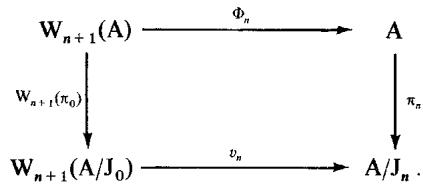
\includegraphics[keepaspectratio]{images/part002_309b7be5.jpg}}

\begin{enumerate}
\def\labelenumi{\alph{enumi})}
\setcounter{enumi}{2}
\tightlist
\item
  置 \(u_n = v_n \circ \mathbf{W}_{n+1}(\overline{\varphi}) \circ \mathbf{F}^{-n}\)。于是，对每个 \(n \in \mathbf{N}\)，下图（其中竖直箭头表示典范投影）是交换的
\end{enumerate}

\pandocbounded{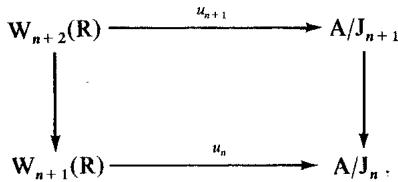
\includegraphics[keepaspectratio]{images/part002_feb0ecf4.jpg}}

\begin{enumerate}
\def\labelenumi{\alph{enumi})}
\setcounter{enumi}{3}
\tightlist
\item
  存在唯一的环同态 u，使下图成为交换的。
\end{enumerate}

\pandocbounded{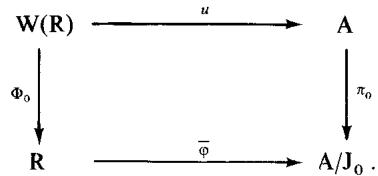
\includegraphics[keepaspectratio]{images/part002_890d1cac.jpg}}

  同态 \(u\) 是连续的（当 \(\mathbf{W}(\mathbf{R})\) 赋有 \(p\)-进拓扑时），且对每个 \(\boldsymbol{a} = (a_n)_{n \in \mathbb{N}} \in \mathbf{W}(\mathbf{R})\)，有 \(u(\boldsymbol{a}) = \sum_{n=0}^{\infty} p^n \varphi(a_n^{p^{-n}})\)。

（\(u\) 的存在性由前述可得。为证明 \(u\) 的唯一性、连续性及其显式表达式，利用等式 \(\varphi = u \circ \tau\)，其中 \(\varphi\) 是 a) 中构造的从 R 到 A 的映射，而 \(\tau: \mathrm{R} \to \mathrm{W(R)}\) 是 § 1, n° 5 中定义的映射。）

\begin{enumerate}
\def\labelenumi{\alph{enumi})}
\setcounter{enumi}{4}
\tightlist
\item
  给出 § 2, n° 4 定理 2 的另一个证明，它不同于正文中的证明，也不同于习题 4, c) 中的证明。
\end{enumerate}

\begin{enumerate}
\def\labelenumi{\arabic{enumi})}
\setcounter{enumi}{6}
\tightlist
\item
  \begin{enumerate}
  \def\labelenumii{\alph{enumii})}
  \tightlist
  \item
    设 R 是特征为 p 的完美环，R' 是特征为 p 的环。设 f 是从 R 到 R' 中的同态。则同态 W(f): W(R) → W(R') 是使下图成为交换的唯一同态。
  \end{enumerate}
\end{enumerate}

\pandocbounded{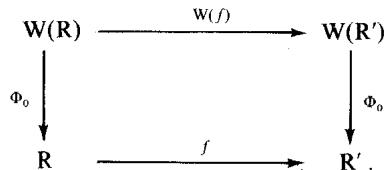
\includegraphics[keepaspectratio]{images/part002_f36acea2.jpg}}

（利用前一习题。）

特别地，取 \(f\) 为 R 上的 p 次幂映射，证明 \(\mathrm{F}_{\mathrm{R}}\) 是 \(\mathbf{W}(\mathbf{R})\) 的使得 \(\Phi_{0} \circ \mathrm{F}_{\mathrm{R}} = f \circ \Phi_{0}\) 的唯一自同态。它由等式

\[
\mathrm{F} _ {\mathbf {R}} (\tau (x)) = \tau (x ^ {p}) \quad \text { for all } \quad x \in \mathbf {R}  .
\]

\begin{enumerate}
\def\labelenumi{\alph{enumi})}
\setcounter{enumi}{1}
\tightlist
\item
  设 A 是对 p-进拓扑分离且完备的环。假设 A 中乘以 \(p.1_{A}\) 的乘法是单射，且 A/pA 是完美环。则存在唯一的 A 的自同态 \(\sigma\)，使得 \(\sigma(x) \equiv x^{p} \mod pA\)（对 \(x \in A\)），且第 44 页习题 14 中所述的同构 \(t_{\sigma}: A \to W(A/pA)\) 的逆由
\end{enumerate}

\[
(a _ {i}) _ {i \in \mathbf {N}} \mapsto \sum_ {i = 0} ^ {\infty} \varphi (a _ {i}) ^ {p ^ {- i}} p ^ {i},
\]

给出，其中 \(\varphi : \mathrm{A} / p\mathrm{A} \to \mathrm{A}\) 是通过过渡到商给出 \(\mathrm{A} / p\mathrm{A}\) 的恒等映射、且满足 \(\varphi(x^p) = \varphi(x)^p\)（对 \(x \in \mathbb{R}\)）的唯一映射（参见习题 6, a)）。

\begin{enumerate}
\def\labelenumi{\arabic{enumi})}
\setcounter{enumi}{7}
\item
  设 C 是以 k 为剩余域的无限长度 p-环。k 的每个自同构都可扩张为 C 的自同构。C 的通过过渡到商在 k 上诱导恒等映射的自同构是恒等映射，当且仅当 k 是完美的。
\item
  设 \(k\) 是特征为 \(p\) 的域，\(\mathbf{C}_k\) 是无限长度的 \(p\)-环（以 \(k\) 为剩余域）。设 A 是分离且完备的局部环，\(u: \mathbf{C}_k \to \mathbf{A}\) 是局部同态，使得由 \(u\) 通过过渡到商得到的同态使 A 的剩余域 K 成为 \(k\) 的可分扩张。设 \(\mathbf{C}_{\mathbf{K}}\) 是以 K 为剩余域的无限长度 \(p\)-环。证明存在局部同态 \(i: \mathbf{C}_k \to \mathbf{C}_{\mathbf{K}}\) 与 \(v: \mathbf{C}_{\mathbf{K}} \to \mathbf{A}\)，使得 \(u = v \circ i\)，且 \(v\) 通过过渡到商在 K 上诱导恒等映射。
\item
  设 \(k\) 是特征为 \(p\) 的域，\((\xi_{\lambda})_{\lambda \in \Lambda}\) 是一个 \(p\)-基（\(k\) 的），且对每个整数 \(n \geqslant 1\)，用 \(C_n\) 表示 \(\mathbf{W}_n(k)\) 的由 \(\mathbf{W}_n(k^{p^{n-1}})\) 与诸元素 \(\tau(\xi_{\lambda}) = [\xi_{\lambda}, 0, ..., 0]\)（\(\lambda \in \Lambda\)）所生成的子环。对每个整数 \(n \geqslant 1\)，\(\mathbf{W}_{n+1}(k)\) 到 \(\mathbf{W}_n(k)\) 上的投影把 \(C_{n+1}\) 映到 \(C_n\) 中。用 C 表示 \(\mathbf{W}(k)\) 的作为诸 \(C_n\) 的逆极限的那个子环。
\end{enumerate}

\begin{enumerate}
\def\labelenumi{\alph{enumi})}
\item
  设 n 是 \(\geqslant 0\) 的整数。置 \(\mathbf{A} = \mathbf{W}_{n+1}(k)\)，并对每个整数 \(i \geqslant 0\)，用 \(\rho_{i} = \rho_{n,i}^{A}\) 表示第 69 页习题 2 中定义的从 k 到 A 的映射。证明对 \(a \in k\)，有 \(\rho_{i}(a) = V^{i}\tau(a^{p^{n}})\)。由此推出，诸元素 \(\rho_{i}(a)\)（\(a \in k\)）生成 A 的子环 \(\mathbf{W}_{n+1}(k^{p^{n}})\)。
\item
  设 \(\tilde{\mathbf{C}}\) 是一个 \(p\)-环（以 \(k\) 为剩余域）且长度无限，\((x_{\lambda})_{\lambda \in \Lambda}\) 是 \(\tilde{\mathbf{C}}\) 中提升 \(p\)-基 \((\xi_{\lambda})_{\lambda \in \Lambda}\) 的元素族。利用第 70 页习题 4 证明：对每个整数 \(n \geqslant 1\)，存在唯一的环同态 \(\varphi_n: \tilde{\mathbf{C}} \to \mathbf{W}_n(k)\)，它通过过渡到商在 \(k\) 上诱导恒等映射，且把 \(x_{\lambda}\) 映到 \(\tau(\xi_{\lambda})\) 上（对每个 \(\lambda \in \Lambda\)）。由第 69 页习题 3 推出，\(\varphi_n\) 的像是 \(\mathbf{C}_n\)。
\item
  诸映射 \((\varphi_n)_{n\geqslant 1}\) 构成从 \(\tilde{\mathbf{C}}\) 到诸 \(C_n\) 中的映射的一个逆系统，且 \(\varphi = \lim \varphi_n\) 是从 \(\tilde{\mathbf{C}}\) 到 C 上的同构。对每个 \(n\geqslant 1\)，典范投影 \(\mathbf{C}\to \mathbf{C}_n\) 把 \(C_n\) 与 \(\mathrm{C} / p^n\mathrm{C}\) 等同起来。
\end{enumerate}

\begin{enumerate}
\def\labelenumi{\arabic{enumi})}
\setcounter{enumi}{10}
\tightlist
\item
  设 \(k\) 是特征为 \(p\) 的域，\((\xi_{\lambda})_{\lambda \in \Lambda}\) 是一个 \(p\)-基（\(k\) 的），\(C\) 是 \(\mathrm{W}(k)\) 的 Cohen 子环，它包含 \(\tau(\xi_{\lambda})\)（对每个 \(\lambda \in \Lambda\)）。设 \((\varepsilon_j)_{j \in J}\) 是 \(k^*/(k^{*p})\) 作为 \(\mathbf{F}_p\)-向量空间的基。设 \(n\) 是 \(\geqslant 0\) 的整数，\((x_j)_{j \in J}\) 是 \(k^*\) 中元素的族，使得 \(x_j\) 在 \(k^*/k^{*p}\) 中的像是 \(\varepsilon_j\)（对所有 \(j \in J\)）。
\end{enumerate}

\begin{enumerate}
\def\labelenumi{\alph{enumi})}
\item
  群 \(k^{*} / k^{*p^{n}}\) 是自由 \((\mathbf{Z} / p^{n}\mathbf{Z})\)-模，以 \((\overline{x}_j)_{j\in J}\) 为基，其中 \(\overline{x}_j\) 是 \(x_j\) 在 \(k^{*} / k^{*p^{n}}\) 中的类。
\item
  对每个 \(j \in J\)，写出 \(x_{j}\) 沿基 \((\xi^{m})_{m \in M_{n}}\)（k 在 \(k^{p^{n}}\) 上的基）的分解（记号见第 69 页习题 3）：
\end{enumerate}

\[
x _ {j} = \sum_ {\boldsymbol {m} \in \mathbf {M} _ {n}} a _ {j, \boldsymbol {m}} ^ {p ^ {n}} \xi^ {\boldsymbol {m}}, \quad a _ {j, \boldsymbol {m}} \in k.
\]

置

\[
\sigma_ {n} (x _ {j}) = \sum_ {m \in \mathbf {M} _ {n}} \tau (a _ {j, m} ^ {p ^ {n}} \xi^ {m}) \quad \text { for all } \quad j \in J
\]

以及

\[
\sigma_ {n} (x) = \tau (x) \quad \text { for } \quad x \in k ^ {* p ^ {n}}.
\]

于是 \(\sigma_{n}\) 以唯一的方式扩张为从 \(k^{*}\) 到 \(\mathrm{C} / p^{n + 1}\mathrm{C}\) 中的乘法映射，仍记作 \(\sigma_{n}\)，它通过过渡到商决定 \(k^{*}\) 到 \(k = \mathrm{C} / p\mathrm{C}\) 中的包含映射。c) 设 \(\sigma_{n}^{\prime}\) 是从 \(k^{*}\) 到 \(\mathrm{C} / p^{n + 1}\mathrm{C}\) 中的另一个乘法映射，它通过过渡到商定义 \(k^{*}\) 到 \(k\) 中的包含映射。则对每个 \(x\in k^{*}\)，有 \(\sigma_{n}(x) = v(x)\sigma_{n}^{\prime}(x)\)，其中 \(v\) 是从 \(k^{*}\) 到乘法群 \((1 + p\mathrm{C}) / (1 + p^{n + 1}\mathrm{C})\) 中的、在 \(k^{*p^n}\) 上平凡的同态。任意一个族 \((\beta_j)_{j\in J}\)（元素属于 \(\mathrm{C} / p^n\mathrm{C}\)）都由公式

\[
v (x _ {j}) = 1 + p \beta_ {j} \quad \text { for all } \quad j \in J.
\]

\begin{enumerate}
\def\labelenumi{\alph{enumi})}
\setcounter{enumi}{3}
\item
  对每个整数 \(n \geqslant 0\) 以及每个乘法映射 \(s_{n}: k^{*} \to C/p^{n+1}C\)（通过过渡到商定义 \(k^{*}\) 到 k 中的包含映射），存在乘法映射 \(s_{n+1}: k^{*} \to C/p^{n+2}C\)，它通过过渡到商决定 \(s_{n}\)。
\item
  证明存在乘法截面 \(s:k\to C\)。可以要求 \(s(\xi_{\lambda})=\tau(\xi_{\lambda})\)（对每个 \(\lambda\in\Lambda\)）。
\end{enumerate}

\(f)\) 设 A 是分离且完备的局部环。设 \(k\) 是其剩余域，\((\xi_{\lambda})_{\lambda \in \Lambda}\) 是一个 \(p\)-基（\(k\) 的），且对 \(\lambda \in \Lambda\)，用 \(a_{\lambda}\) 表示 \(\xi_{\lambda}\) 在 A 中的一个提升。证明存在乘法截面 \(k^{*} \to A\)，满足 \(s(\xi_{\lambda}) = a_{\lambda}\)。

\begin{enumerate}
\def\labelenumi{\arabic{enumi})}
\setcounter{enumi}{11}
\tightlist
\item
  设 A 是剩余域特征为 p 的完备局部环。
\end{enumerate}

\begin{enumerate}
\def\labelenumi{\alph{enumi})}
\item
  设 \(x \in \mathfrak{m}_{\mathrm{A}}\)。映射 \(n \mapsto (1 + x)^n\)（从 \(\tilde{\mathbf{Z}}\) 到 \(1 + \mathfrak{m}_{\mathrm{A}}\)）唯一地扩张为从 \(\mathbf{Z}_p\) 到 \(1 + \mathfrak{m}_{\mathrm{A}}\) 中的连续映射，记作 \(\alpha \mapsto (1 + x)^{\alpha}\)。这样就定义了一个 \(\mathbf{Z}_p\)-模结构，作用在乘法群 \(1 + \mathfrak{m}_{\mathrm{A}}\) 上。
\item
  用 \(\delta\) 表示第 68 页习题 58 中的形式级数 \(\exp\left(-\sum_{n=0}^{\infty}\mathrm{T}^{p^n}/p^n\right)\)。映射 \(x \mapsto \delta(x)\)（从 \(\mathfrak{m}_{\mathrm{A}}\) 到 \(1 + \mathfrak{m}_{\mathrm{A}}\)）是双射。
\item
  设 \(k\) 是特征为 \(p\) 的完美域，\(\varphi\) 是从 \(\mathbf{W}(k)\) 到 A 中的局部同态。对 \(\alpha \in \mathbf{W}(k)\)，考察级数 \(\varphi \mathrm{E}_{\mathrm{F}}(\alpha, \mathrm{T})\)，它是由 \(\varphi\) 作用于第 68 页习题 58 f) 中的级数 \(\mathrm{E}_{\mathrm{F}}(\alpha, \mathrm{T})\) 的系数而得到的。对 \(\alpha \in \mathbf{W}(k)\)，\(x \in 1 + m_{\mathbf{A}}\)，置 \(x^{\alpha} = \varphi \mathrm{E}_{\mathrm{F}}(\alpha, \xi^{-1}(x))\)。证明这定义了加法群 \(\mathbf{W}(k)\) 在集合 \(1 + m_{\mathbf{A}}\) 上的一个作用，它扩张了 a) 中定义的 \(\mathbf{W}(\mathbf{F}_p)\)（等同于 \(\mathbf{Z}_p\)）的作用。证明对 \(a \in \mathbf{Z}_p\)，\(\alpha \in \mathbf{W}(k)\)，\(x \in 1 + m_{\mathbf{A}}\)，还有关系式 \((x^{\alpha})^{a} = x^{a\alpha}\)。
\item
  利用第 44 页习题 15 证明：对 \(a \in \mathbf{Z}_{p}\)、\(\alpha \in \mathbf{W}(k)\) 与 \(x \in 1 + m_{\mathbf{A}}\)，关系式 \((x^{a})^{\alpha} = x^{a\alpha}\) 并不总成立。同样，对 \(\alpha \in \mathbf{W}(k)\) 以及 \(x, y\)（属于 \(1 + m_{\mathbf{A}}\)），关系式 \((xy)^{\alpha} = x^{\alpha}y^{\alpha}\) 也不总成立。
\end{enumerate}

\begin{enumerate}
\def\labelenumi{\arabic{enumi})}
\setcounter{enumi}{12}
\tightlist
\item
  设 A 是特征为零的完备离散赋值环，其剩余域的特征为 \(p\)。设 K 是 A 的分式域，\(\overline{\mathbf{K}}\) 是 K 的一个代数闭包，赋以延拓 K 的赋值的唯一赋值 \(v\)（VI, § 8, n° 7），\(\hat{\mathbf{K}}\) 是 \(\overline{\mathbf{K}}\) 的完备化，\(\hat{\mathbf{A}}\) 是 \(\hat{\mathbf{K}}\) 的赋值环。置 \(e = v(p)\)。
\end{enumerate}

\begin{enumerate}
\def\labelenumi{\alph{enumi})}
\tightlist
\item
  级数 \(\log(1 + x) = \sum_{i=1}^{\infty} (-1)^{i-1} x^i / i\) 对 \(v(x) > 0\) 收敛，并定义 \(\mathbf{Z}_p\)-模的同态（参见习题 12）
\end{enumerate}

\[
\begin{array}{l} \log : 1 + \mathfrak {m} _ {\hat {\mathbf {A}}} \to \hat {\mathbf {K}}, \\ \log : 1 + \mathfrak {m} _ {\mathbf {A}} \to \mathbf {K}. \end{array}
\]

\begin{enumerate}
\def\labelenumi{\alph{enumi})}
\setcounter{enumi}{1}
\tightlist
\item
  级数 \(\exp(x) = \sum_{i=0}^{\infty} x^{i}/i!\) 在理想 \(a\)（\(\hat{K}\) 的，由赋值 \(>e/(p-1)\) 的元素组成）上收敛，并定义 \(\mathbf{Z}_{p}\)-模的同态
\end{enumerate}

\[
\begin{array}{l} \exp : a \to 1 + m _ {\hat {A}} \\ \exp : a \cap K \to 1 + m _ {A}. \end{array}
\]

\begin{enumerate}
\def\labelenumi{\alph{enumi})}
\setcounter{enumi}{2}
\tightlist
\item
  对 \(x \in \mathfrak{a}\)，有 \(\log(\exp(x)) = x\)，\(\log(1 + x) \in \mathfrak{a}\)，以及 \(\exp(\log(1 + x)) = 1 + x\)。于是 exp 定义 \(\mathbf{Z}_p\)-模的同构
\end{enumerate}

\[
\begin{array}{l}\mathfrak {a} \rightarrow 1 + \mathfrak {a}\\\mathfrak {a} \cap \mathbf {K} \rightarrow 1 + (\mathfrak {a} \cap \mathbf {K})\end{array}
\]

其对逆由 log 定义。

\begin{enumerate}
\def\labelenumi{\alph{enumi})}
\setcounter{enumi}{3}
\tightlist
\item
  log 在 \(1 + m_{\hat{A}}\) 上的核由阶为 p 的幂的单位根组成。像 \(\log(1 + m_{\hat{A}})\) 等于 \(m_{\hat{A}}\)。
\end{enumerate}

\begin{enumerate}
\def\labelenumi{\arabic{enumi})}
\setcounter{enumi}{13}
\tightlist
\item
  设 A 是特征为零的完备离散赋值环，其剩余域 \(k\) 是特征为 \(p\) 的完美域。设 K 是 A 的分式域。设 \(n\) 是 \(\geqslant 1\) 的整数，\(\zeta\) 是 K 中一个本原 \(p^n\)-次单位根。设 \(\overline{\mathbf{K}}\) 是 K 的一个代数闭包，赋以延拓 K 的赋值的唯一赋值 \(v\)。
\end{enumerate}

\begin{enumerate}
\def\labelenumi{\alph{enumi})}
\item
  用 C 表示 A 的 Cohen 子环，T 表示其分式域；它是 K 的一个子域。从 W(k) 到 C 的典范同构诱导从 \(W(k) \otimes_{\mathbb{Z}} \mathbb{Q}\) 到 T 的一个同构。对 k 的每个有限扩张 l，域 \(W(l) \otimes_{\mathbb{Z}} \mathbb{Q}\) 是 \(W(k) \otimes_{\mathbb{Z}} \mathbb{Q}\) 的有限扩张，且当 l 是 Galois 扩张时它也是 Galois 的。若 l 是 Galois 的，T 的唯一扩张 \((T_l)\)（\(\overline{\mathbf{K}}\) 中同构于 \(W(l) \otimes_{\mathbb{Z}} \mathbb{Q}\) 的那个）的剩余域同构于 l。特别地，当 l 取遍 k 的有限 Galois 扩张（在 k 的一个固定代数闭包中）时，并 \(T_{\infty}\)（诸域 \((T_l)\) 的并）以 k 的一个代数闭包 \(\overline{k}\) 为其剩余域。对 K 同样成立。对 \(\overline{k}\) 中 k 的每个扩张 l，用 \((T_l)\) 表示 \(T_{\infty}\) 中剩余域为 \(\overline{k}\) 的子域 l 的 T 的唯一扩张，并用 \((K_l)\) 表示 K 与 \((T_l)\) 的合成。于是，若 l 在 k 上是 Galois 的，则 \((K_l)\) 在 K 上是 Galois 的，且其 Galois 群典范地等同于 l 在 k 上的 Galois 群。
\item
  用 \(k_n\) 表示 \(k\) 在 \(\overline{k}\) 中的其 Galois 群被 \(p^n\) 零化的最大交换扩张。根据第 45 页习题 19，我们有典范同构
\end{enumerate}

\[
\operatorname{Gal} (k _ {n} / k) \to \operatorname{Hom} (\mathrm{W} _ {n} (k) / \wp \mathrm{W} _ {n} (k), \mathbf {Z} / p ^ {n} \mathbf {Z}).
\]

由 A, V, 第 85 页定理 4，我们有典范同构

\[
\operatorname{Gal} \left(\mathrm{K} _ {k _ {n}} / \mathrm{K}\right)\rightarrow \operatorname{Hom} \left(\mathrm{H} _ {n} / \mathrm{K} ^ {* p ^ {n}}, \mu_ {p _ {n}} (\mathrm{K})\right)
\]

\(\text{其中 }\mathbf{H}_n = (\mathbf{K}_{\overline{k}}^*)^{p^n}\cap \mathbf{K}^*\)

证明存在唯一的映射

\[
\mathrm{E} ^ {*}: \mathrm{W} _ {n} (k) / \wp \mathrm{W} _ {n} (k) \rightarrow \mathrm{H} _ {n} / \mathrm{K} ^ {* p ^ {n}}
\]

使得下图交换：

\[
\begin{array}{c} \operatorname{Gal} (K _ {k _ {n}} / K) \xrightarrow {} \operatorname{Hom} (H _ {n} / K ^ {* p ^ {n}}, \mu_ {p ^ {n}} (K)) \\ \Bigg \downarrow \\ \operatorname{Gal} (k _ {n} / k) \xrightarrow {} \operatorname{Hom} (W _ {n} (k) / \wp W _ {n} (k), Z / p ^ {n} Z), \end{array}
\]

其中右侧的竖直箭头表示这样的映射：它把同态 \(\varphi\)（从 \(\mathbf{H}_n / \mathbf{K}^{*p^n}\) 到 \(\mu_{p^n}(\mathbf{K})\) 中的）映为同态 \(\psi\)（从 \(\mathrm{W}_n(k) / \wp\mathrm{W}_n(k)\) 到 \(\mathbf{Z} / p^n\mathbf{Z}\) 中的），后者由 \(\zeta^{\psi (\alpha)} = \varphi (\mathrm{E}^{*}(\alpha))\)（对 \(\alpha \in \mathrm{W}_n(k) / \wp\mathrm{W}_n(k)\)）定义。映射 \(\mathrm{E}^*\) 是同构。

\begin{enumerate}
\def\labelenumi{\arabic{enumi})}
\setcounter{enumi}{14}
\tightlist
\item
  保留前一习题的假设与记号。
\end{enumerate}

\begin{enumerate}
\def\labelenumi{\alph{enumi})}
\tightlist
\item
  设 \(\alpha \in \mathbf{W}(k)\)，\(\overline{\alpha} \in \mathbf{W}(\overline{k})\) 满足 \(p(\overline{\alpha}) = \alpha\)（参见第 45 页习题 19）。则元素 \(\zeta^{p^{n\overline{\alpha}}}\)（第 72 页习题 12）作为 \(\widehat{\mathbf{K}}\)（\(\overline{\mathbf{K}}\) 的完备化）的元素只依赖于 \(\alpha\)，属于 \(\mathbf{K}\)，并且我们有
\end{enumerate}

\[
v \left(\zeta^ {p ^ {n} \bar {\alpha}} - 1\right) \geqslant e p / (p - 1) \quad (\text { with } e = v (p)).
\]

（可以证明等式

\[
\log \left(\zeta^ {p ^ {n} \overline {{{\alpha}}}}\right) = - p ^ {n} \sum_ {j = 1} ^ {\infty} \sum_ {\sigma = 0} ^ {j - 1} \left(\mathrm{F} ^ {\sigma} \alpha\right) \frac {\pi^ {p ^ {j}}}{p ^ {j}}
\]

\(\text{其中 }\pi = \delta^{-1}(\zeta)\)（出处同上），其中 F 表示 \(\mathbf{W}(k)\) 的 Frobenius 自同构。）

\begin{enumerate}
\def\labelenumi{\alph{enumi})}
\setcounter{enumi}{1}
\tightlist
\item
  对 \(\alpha \in \mathbf{W}(k)\)，用 \(\mathrm{E}^{**}(\alpha)\) 表示 \(\mathrm{K}^* / \mathrm{K}^{*p^n}\) 中 \(\zeta^{p^n\overline{\alpha}}\) 的类。则 \(\mathrm{E}^{**}(\alpha)\) 等于 1（若 \(\alpha \in p\mathbf{W}(k)\) 或 \(\alpha \in p^n\mathbf{W}(k)\)）。从 \(\mathrm{W}_n(k)/\wp\mathrm{W}_n(k)\) 到 \(\mathrm{K}^* / \mathrm{K}^{*p^n}\) 中的、把 \(\alpha \in \mathbf{W}(k)\) 的类映为元素 \(\mathrm{E}^{**}(\alpha)\) 的映射取值在 \(\mathrm{H}_n / (\mathrm{K}^*)^{p^n}\) 中，且满足习题 14 b) 的条件。
\end{enumerate}

\begin{enumerate}
\def\labelenumi{\arabic{enumi})}
\setcounter{enumi}{15}
\tightlist
\item
  设 A 是以 k 为剩余域的完备离散赋值环。
\end{enumerate}

\begin{enumerate}
\def\labelenumi{\alph{enumi})}
\item
  证明存在乘法截面 \(\varphi:k^{*}\to\mathring{\mathrm{A}}\)。（若 A 包含一个域，利用 § 3。否则，利用第 72 页习题 11。）
\item
  设 \(t\) 是 A 的一个单值化元，\(\mathcal{C}\) 是由 \(t\) 生成的群，\(\varphi:k^{*}\to A\) 是一个乘法截面。A 的分式域的乘法群分解为直积 \(\mathcal{C}\times\varphi(k^{*})\times(1+\mathfrak{m}_{\mathbf{A}})\)。
\item
  假设 A 是等特征的，并设 K 是一个系数域。则 A 等同于系数在 K 中的形式级数环 K{[}{[}T{]}{]}，且群 1 + m\_A 等同于群 \(\Lambda(K) = 1 + TK[[T]]\)（参见第 56 页习题 42）。若 K 的特征为零，则映射 \(\varphi \mapsto \frac{1}{T} \log \varphi\)（从群 \(\Lambda(K)\) 到加法群 \(K[[T]]\) 的）是同构。若 A 的特征为 \(p, 1 + m_A\)，则它等同于群 \(W(A)^L\)，其中 L 是与 \(p\) 互素的正整数的集合（利用第 54 页习题 40 \(h\) ) 与第 57 页习题 43 \(b\) )）。
\end{enumerate}

\begin{enumerate}
\def\labelenumi{\arabic{enumi})}
\setcounter{enumi}{16}
\tightlist
\item
  设 A 是完备离散赋值环，其剩余域 k 是特征为 p 的完美域，其分式域的特征为 0。设 f 是从 W(k) 到 A 的、在剩余域 k 上诱导恒等映射的唯一同态。最后，设 π 是 A 的一个单值化元。
\end{enumerate}

\begin{enumerate}
\def\labelenumi{\alph{enumi})}
\item
  存在系数在 \(f(\mathbf{W}(k))\) 中的 Eisenstein 多项式 P，使得 \(\mathbf{P}(\pi)=0\)（利用 VIII, § 5, n° 4）。
\item
  用 \(e\) 表示 \(p\) 的赋值。对每个整数 \(n \geqslant 0\)，用 \(U_n\) 表示乘法群 \(1 + m_A^n\)，并置 \(\lambda(n) = \inf(np, n + e)\)，\(e_1 = e/(p - 1)\)。设 \(u\) 是 \(k^*\) 中元素 \(p\pi^{-e}\) 的类。用 \(\varphi\) 表示 \(U_1\) 的把 \(x\) 映为 \(x^p\) 的自同态。于是，对每个整数 \(n \geqslant 1\)，有 \(\varphi(U_n) \subset U_{\lambda(n)}\)，\(\varphi(U_{n+1}) \subset U_{\lambda(n)+1}\)，且诱导同态 \(\varphi_n: U_n/U_{n+1} \to U_{\lambda(n)}/U_{\lambda(n)+1}\) 当 \(n \neq e_1\) 时是同构。若 \(n = e_1\)，则 \(\varphi_n\) 是单射当且仅当方程 \(x^{p-1} + u = 0\) 在 \(k\) 中无解，且是满射当且仅当方程 \(x^p + ux = y\) 在 \(k\) 中有解（对每个 \(y \in k\)）。
\item
  下列两个条件等价：
\end{enumerate}

\begin{enumerate}
\def\labelenumi{(\roman{enumi})}
\item
  A 包含 p 次单位根；
\item
  \(e_1\) 是整数且方程 \(x^{p - 1} + u = 0\) 在 \(k\) 中有一个解。
\end{enumerate}

\begin{enumerate}
\def\labelenumi{\alph{enumi})}
\setcounter{enumi}{3}
\item
  A 的拓扑在 \(\mathbf{U}_1\) 上诱导的拓扑与 \(\mathbf{U}_1\) 的 p-进拓扑一致。
\item
  用 S 表示由整数 \(n \geqslant 1\)（使 A 包含 \(p^n\)-次单位根）组成的集合。则 \(s = \text{Card}(S)\) 是有限的。
\item
  用 I 表示整数 \(i\)（与 \(p\) 互素且满足 \(1 \leqslant i < e + e_1\)）组成的集合。则有 Card(I) = \(e\)，且 \(\mathbf{N} - \{0\}\) 在 \(\lambda\) 之下的像是 \(\mathbf{N} - (\mathbf{I} \cup \{0\})\)。
\item
  若 \(e_1\) 是整数且 \(\varphi_{e_1}\) 不是满射，则置 \(\mathbf{I}' = \mathbf{I} \cup \{e + e_1\}\)；否则置 \(\mathbf{I}' = \mathbf{I}\)。对每个整数 \(i \in \mathbf{I}'\)，用 \(\pi_i\) 表示 A 中赋值为 \(i\) 的一个元素。则从 \(\mathbf{W}(k)^{\mathbf{I}'}\) 到 \(\mathbf{U}_1\) 中的、把 \((a_i)_{i \in \mathbf{I}'}\) 映为 \(\prod_{i \in \mathbf{I}'} (1 + \pi_i)^{a_i}\) 的映射是满射；它是
\end{enumerate}

\(\mathbf{Z}_{p}\)-模的一个同态。

\(h)\) 设 \(n\) 是 \(>e_{1}\) 的整数，\(\mathbf{I}(n)\) 是区间 \([n, \lambda(n) - 1]\)（\(\mathbf{N}\) 的）。对每个整数 \(i \in \mathbf{I}(n)\)，用 \(\pi_{i}\) 表示 \(\mathbf{A}\) 中赋值为 \(i\) 的一个元素。则从 \(\mathbf{W}(k)^{\mathbf{I}(n)}\) 到 \(\mathbf{U}_{n}\) 的、把 \((a_{i})_{i \in \mathbf{I}(n)}\) 映为 \(\prod_{i \in \mathbf{I}(n)} (1 + \pi_{i})^{a_{i}}\) 的映射是 \(\mathbf{Z}_{p}\)-模的同构。

\begin{enumerate}
\def\labelenumi{\roman{enumi})}
\tightlist
\item
  假设 \(k\) 有限，并用 \(d\) 表示 A 的分式域在 \(\mathbf{Q}_{p}\) 上的次数。则 \(\mathbf{Z}_{p}\)-模 \(1 + m_{\mathbf{A}}\) 同构于 \((\mathbf{Z}/p^{s}\mathbf{Z}) \times \mathbf{Z}_{p}^{d}\)。（可利用前面各问，也可利用第 73 页习题 13。）
\end{enumerate}

\exercisesection{代表域}

\begin{enumerate}
\def\labelenumi{\arabic{enumi})}
\tightlist
\item
  设 \(p\) 是素数，\(G\) 是以 \(X\)、\(Y\) 两个生成元生成的自由群，\(F_p[G]\) 是 \(G\) 在 \(F_p\) 上的群代数。置 \(Z = XY - YX\)，并用 \(\mathfrak{a}\) 表示 \(F_p[G]\) 的由元素 \(ZX - XZ\)、\(ZY - YZ\) 与 \(Z^2\) 生成的双边理想。置 \(A = F_p[G]/\mathfrak{a}\)，并用 \(\mathfrak{z}\) 表示 \(A\) 的由 \(Z\) 在 \(A\) 中的像生成的双边理想（我们把 \(X\)、\(Y\)、\(Z\) 在 \(A\) 中的像仍记作 \(X\)、\(Y\)、\(Z\)）。a) 设 \(a\) 是 \(A\) 的一个元素。证明存在两个由 \(F_p\) 的元素组成的有限支撑族，即 \((p_{\alpha,\beta})_{(\alpha,\beta)\in\mathbf{Z}^2}\) 与 \((q_{\alpha,\beta})_{(\alpha,\beta)\in\mathbf{Z}^2}\)，它们由条件
\end{enumerate}

\[
a = \sum_ {(\alpha , \beta) \in \mathbf {Z} ^ {2}} (p _ {\alpha , \beta} + q _ {\alpha , \beta} \mathbf {Z}) \mathrm{X} ^ {\alpha} \mathrm{Y} ^ {\beta}.
\]

唯一确定。由此推出商代数 \(A/\mathfrak{z}\) 是交换的且是整的，并且理想 \(\mathfrak{z}\) 包含在 A 的中心中。

\begin{enumerate}
\def\labelenumi{\alph{enumi})}
\setcounter{enumi}{1}
\tightlist
\item
  对 A 的元素的每个偶 \((a, b)\)，存在 A 的元素 c，使得
\end{enumerate}

\[
  a ^ {k} b - b a ^ {k} = k a ^ {k - 1} c Z \quad \text { for every integer } k \geqslant 0.
\]

由此推出，A 的元素的 p 次幂所成的集合 \(A^{p}\) 包含在 A 的中心中。

\begin{enumerate}
\def\labelenumi{\alph{enumi})}
\setcounter{enumi}{2}
\tightlist
\item
  乘性部分 \(S = A - \mathfrak{z}\)（\(A\) 的）允许在右边与在左边做分式（II, § 2, 习题 22）。用 B 表示这样构造的 \(A\) 的分式环。
\end{enumerate}

（例如，为验证对 A 中的每个 \(a\) 与 S 中的每个 \(s\)，存在 \(b \in A\) 与 \(t \in S\) 使得 \(at = sb\)，可取 \(b = s^{p-1}a\)，\(t = s^p\)，并利用 b)。）

\begin{enumerate}
\def\labelenumi{\alph{enumi})}
\setcounter{enumi}{3}
\item
  证明从 A 到 B 的典范映射是单射。（注意这个映射的核包含在 \(\mathfrak{z}\) 中，并按 a) 的方式推理。）
\item
  B 的中心包含 Z。若 m 是 B 的由 Z 生成的双边理想，则 \(m^{2} = 0\)。
\item
  理想 m 是 B 的不可逆元素的集合，且域 B/m 同构于域 \(\mathbf{F}_{p}(\mathbf{X}, \mathbf{Y})\)。
\item
  证明 B 中不存在其在 B/m 中的像为整个 B/m 的子域。
\end{enumerate}

在习题 2 至 5 中，假设（交换）拓扑环都是线性拓扑化的。若 A 与 B 是两个拓扑环，且 B 是 A-代数，则当定义代数结构的从 A 到 B 的同态为连续时，称 B 是拓扑 A-代数。

\begin{enumerate}
\def\labelenumi{\arabic{enumi})}
\setcounter{enumi}{1}
\tightlist
\item
  设 A 是拓扑环，B 是拓扑 A-代数。我们称 B 是形式光滑 A-代数\(^{1}\)，如果对每个离散拓扑 A-代数 C、C 的每个平方为零的理想 j 以及每个连续 A-同态 \(u: B \to C/j\)，存在通过过渡到商诱导 u 的连续 A-同态 \(v: B \to C\)。
\end{enumerate}

设 A 是环，B 是 A-代数。如果当 A 与 B 赋有离散拓扑时 B 是形式光滑 A-代数，则称 B 是光滑 A-代数。

\begin{enumerate}
\def\labelenumi{\alph{enumi})}
\item
  设 A 是拓扑环，B 是形式光滑 A-代数。设 C 是环，j 是 C 的理想。给 C 赋以 j-进拓扑，并假设 C 对这一拓扑是分离的且完备的。则对每个连续 A-同态 \(u:B\to C/\mathfrak{j}\)，存在连续 A-同态 \(v:B\to C\)，它通过过渡到商诱导 \(u\)。
\item
  设 A 是环。A 上的每个多项式代数都是光滑 A-代数。
\item
  设 A 是拓扑环。若 B 是形式光滑 A-代数，且 C 是形式光滑 B-代数，则 C 是形式光滑 A-代数。
\item
  设 A 是拓扑环，B 是形式光滑 A-代数，A' 是拓扑 A-代数。则拓扑 A'-代数 \(B \otimes_{A} A'\)（III, § 2, 习题 28）是形式光滑 A'-代数。
\item
  设 A 是拓扑环，B 是形式光滑 A-代数。设 S（相应地 T）是 A（相应地 B）的乘性子集，使得 S 在 B 中的像包含于 T。则 \(T^{-1}B\) 是形式光滑 \(S^{-1}A\)-代数（\(T^{-1}B\) 与 \(S^{-1}A\) 的拓扑见 III, § 2, 习题 27）。
\item
  设 n 是 \(\geqslant 1\) 的整数，\((\mathbf{B}_{i})_{1\leqslant i\leqslant n}\) 是拓扑 A-代数的一个族。要使 \(\prod_{i=1}^{n} B_{i}\) 是形式光滑 A-代数，必须且只需 \(B_{i}\) 对 \(1 \leqslant i \leqslant n\) 都是形式光滑 A-代数。
\item
  设 A 是拓扑环，B 是拓扑 A-代数，\(\hat{A}\) 与 \(\hat{B}\) 分别是 A 与 B 的分离完备化。则下列三个条件等价：
\end{enumerate}

\begin{enumerate}
\def\labelenumi{(\roman{enumi})}
\item
  B 是形式光滑 A-代数；
\item
  \(\hat{\mathbf{B}}\) 是形式光滑 A-代数；
\item
  \(\hat{\mathbf{B}}\) 是形式光滑 \(\hat{\mathbf{A}}\)-代数。
\end{enumerate}

\(h)\) 重新采用 \(e\)) 中的记号与假设。则 \(\mathbf{B}\{\mathrm{T}^{-1}\}\) 是形式光滑 \(\mathbf{A}\{\mathrm{S}^{-1}\}\)-代数。

\begin{enumerate}
\def\labelenumi{\arabic{enumi})}
\setcounter{enumi}{2}
\tightlist
\item
  设 \(k\) 是域，A 是交换 \(k\)-代数。对每个整数 \(i \geqslant 1\)，置 \(\mathbf{B}_i = \underbrace{\mathbf{A} \otimes_k \mathbf{A} \otimes_k \cdots \otimes_k \mathbf{A}}_{i \text{ 项}}\)，并给 \(\mathbf{B}_i\) 赋以让
\end{enumerate}

A 作用在第一个分量上所得到的 A-代数结构。置 \(C_{1} = B_{2}\)，\(C_{2} = B_{3}\)，\(C_{3} = B_{4} \oplus B_{3}\)，并用公式定义 A-线性映射 \(d_{2}:C_{2} \to C_{1}\) 与 \(d_{3}:C_{3} \to C_{2}\)

\[
d _ {3} ((1 \otimes x \otimes y \otimes z, 1 \otimes \alpha \otimes \beta)) = x \otimes y \otimes z - 1 \otimes x y \otimes z + 1 \otimes x \otimes y z - z \otimes x \otimes y + 1 \otimes \alpha \otimes \beta - 1 \otimes \beta \otimes \alpha,
\]

\[
d _ {2} (1 \otimes \alpha \otimes \beta) = \alpha \otimes \beta - 1 \otimes \alpha \beta + \beta \otimes \alpha ,
\]

\(^{1}\) 若 A 是（离散）域 k 上的局部的 Noether 的完备代数，则根据下面的习题 5，这一定义与第 VIII 卷第 98 页习题 30 中给出的定义一致。

对 A 的元素 \(x, y, z, \alpha, \beta\) 的任意选择，这样就得到一个 A-模的复形

\[
\mathrm{C} _ {k} (\mathrm{A}): \mathrm{C} _ {3} \xrightarrow {d _ {3}} \mathrm{C} _ {2} \xrightarrow {d _ {2}} \mathrm{C} _ {1}.
\]

若 N 是 A-模，则称 \(k\)-双线性映射 \(f: \mathbf{A} \times \mathbf{A} \to \mathbf{N}\) 为 2-上闭链，如果有恒等式 \(xf(y, z) - f(xy, z) + f(x, yz) - zf(x, y) = 0\)（对 A 中的 \(x, y, z\)）；称它是对称的，如果有 \(f(x, y) = f(y, x)\)（对每个偶 \((x, y) \in \mathbf{A} \times \mathbf{A}\)）。

\begin{enumerate}
\def\labelenumi{\alph{enumi})}
\tightlist
\item
  下列条件等价：
\end{enumerate}

\begin{enumerate}
\def\labelenumi{(\roman{enumi})}
\item
  复形 \(\operatorname{Hom}_{\mathbf{A}}(\mathbf{C}_k(\mathbf{A}), \mathbf{N})\) 对每个 A-模 \(\mathbf{N}\) 都是零调的；
\item
  对每个 A-模 N，每个对称 2-上闭链 \(f:A\times A\to\mathbf{N}\) 都是 1-上边缘，即形如 \(f(a,b)=ag(b)+bg(a)-g(ab)\)，其中 \(g\in\mathrm{Hom}_{k}(\mathbf{A},\mathbf{N})\)；
\item
  A 是 k 上的光滑代数。
\end{enumerate}

\begin{enumerate}
\def\labelenumi{\alph{enumi})}
\setcounter{enumi}{1}
\tightlist
\item
  若 A 是域，则前面的条件还等价于复形 \(C_{k}(A)\) 零调这一条件。
\end{enumerate}

\begin{enumerate}
\def\labelenumi{\arabic{enumi})}
\setcounter{enumi}{3}
\tightlist
\item
  \begin{enumerate}
  \def\labelenumii{\alph{enumii})}
  \tightlist
  \item
    设 \(k\) 是域，\(K\) 是 \(k\) 的一个扩张。若 \(K\) 在 \(k\) 上可分，则 \(K\) 是光滑 \(k\)-代数。（若 \(K\) 是 \(k\) 的有限生成扩张，利用 § 3, n° 2 命题 1。一般情形，把 \(K\) 写成 \(k\) 的有限生成扩张的并，并利用前一习题。）
  \end{enumerate}
\end{enumerate}

\begin{enumerate}
\def\labelenumi{\alph{enumi})}
\setcounter{enumi}{1}
\tightlist
\item
  设 A 是包含域 k 的分离且完备的局部环。利用 a)，证明 A 有一个表示域。若 A 的剩余域是 k 的可分扩张，则 A 有一个包含 k 的表示域。
\end{enumerate}

\begin{enumerate}
\def\labelenumi{\arabic{enumi})}
\setcounter{enumi}{4}
\tightlist
\item
  设 A 是包含域 \(k\) 的 Noether 局部环，m 是 A 的极大理想。假设 A 是形式光滑 \(k\)-代数（域 \(k\) 是离散的）。
\end{enumerate}

\begin{enumerate}
\def\labelenumi{\alph{enumi})}
\item
  设 K 是环 \(\mathbb{A}/\mathfrak{m}^2\) 的一个表示域（习题 4 b)），\(x_1, \ldots, x_d\) 是 m 中其像构成 K-向量空间 \(\mathfrak{m}/\mathfrak{m}^2\) 之基的元素。设 \(\mathrm{K}[\mathrm{X}_1, \ldots, \mathrm{X}_d]\) 是 \(d\) 个未定元 \(\mathrm{X}_1, \ldots, \mathrm{X}_d\) 的多项式环，\(\mathfrak{n}\) 是它由 \(\mathrm{X}_1, \ldots, \mathrm{X}_d\) 生成的理想，\(\varphi\) 是从 \(\mathrm{K}[\mathrm{X}_1, \ldots, \mathrm{X}_d]\) 到 \(\mathbb{A}/\mathfrak{m}^2\) 中的、把 \(\mathrm{X}_i\) 映到 \(x_i\)（\(1 \leqslant i \leqslant d\)） 且在 K 上诱导恒等映射的同态。则 \(\varphi\) 诱导同构 \(\overline{\varphi}\)（从 \(\mathrm{K}[\mathrm{X}_1, \ldots, \mathrm{X}_d]/\mathfrak{n}^2\) 到 \(\mathbb{A}/\mathfrak{m}^2\) 上的）。
\item
  对每个整数 \(n \geqslant 1\)，存在同态 \(\psi_n: \mathbb{A} \to \mathrm{K}[\mathrm{X}_1, \ldots, \mathrm{X}_d]/\mathfrak{n}^{n+1}\)，它通过过渡到商诱导 \(\overline{\varphi}^{-1}\)。这样的同态 \(\psi_n\) 是满射。
\item
  对每个整数 \(n \geqslant 1\)，A-模 \(\mathbf{A} / \mathfrak{m}^{n+1}\) 的长度至少为 \(\binom{d+n}{d}\)，且有 \(\dim(\mathbf{A}) \geqslant d\)。
\item
  对 \(k'\)（\(k\) 的每个有限扩张）以及每个极大理想 \(m'\)（半局部环 \(A \otimes_k k'\) 的），局部环 \((A \otimes_k k')_{m'}\) 都是正则的。
\end{enumerate}

\begin{enumerate}
\def\labelenumi{\arabic{enumi})}
\setcounter{enumi}{5}
\tightlist
\item
  设 \(k\) 是域，\(K\) 是 \(k\) 的一个扩张。假设 \(K\) 是光滑 \(k\)-代数。设 \(k'\) 是 \(k\) 的有限次数代数扩张。
\end{enumerate}

\begin{enumerate}
\def\labelenumi{\alph{enumi})}
\item
  环 K \(\otimes_{k} k'\) 是有限多个 Artin 局部环的乘积，这些局部环都是光滑 \(k'\)-代数（利用第 76 页习题 2）。
\item
  环 K \(\otimes_{k} k'\) 是既约的（利用前一习题）。
\item
  域 K 在 k 上是可分的。
\end{enumerate}

\begin{enumerate}
\def\labelenumi{\arabic{enumi})}
\setcounter{enumi}{6}
\tightlist
\item
  设 \(k\) 是域，\(P\) 是其素子域，\(K\) 是 \(k\) 的一个扩张。则下列条件等价：
\end{enumerate}

\begin{enumerate}
\def\labelenumi{\alph{enumi})}
\item
  k 到 K-模 M 中的每个导子都唯一地扩张为 K 到 M 中的导子。
\item
  我们有 \(\Omega_{\mathbf{P}}(\mathbf{K}) = \Omega_{\mathbf{P}}(k)\otimes_k\mathbf{K}\)。
\item
  域 K 在 k 上可分，且 \(\Omega_{k}(\mathbf{K}) = 0\)。
\end{enumerate}

若 \(k\) 的特征为 0，则这些条件还等价于条件：

\begin{enumerate}
\def\labelenumi{\alph{enumi})}
\setcounter{enumi}{3}
\tightlist
\item
  域 K 是 k 的代数扩张。
\end{enumerate}

若 \(k\) 的特征 \(p\ne0\)，则它们还等价于条件：

\begin{enumerate}
\def\labelenumi{\alph{enumi})}
\setcounter{enumi}{4}
\item
  \(\mathbf{K} = k\otimes_{k^p}\mathbf{K}^p.\)
\item
  k 的每个 p-基也是 K 的 p-基。
\end{enumerate}

\begin{enumerate}
\def\labelenumi{\arabic{enumi})}
\setcounter{enumi}{7}
\tightlist
\item
  设 \(k\) 是域，\(K\) 是 \(k\) 的一个扩张。我们称 \(K\) 在 \(k\) 上是形式平展的，如果对每个 \(k\)-代数 \(A\)、每个平方为零的理想 \(a\)（\(A\) 的）以及每个 \(k\)-同态 \(u:K\to A/a\)，存在唯一的 \(k\)-同态 \(v:K\to A\)，它通过过渡到商给出 \(u\)。
\end{enumerate}

\begin{enumerate}
\def\labelenumi{\alph{enumi})}
\item
  若 K 在 k 上形式平展，则前一习题的诸等价条件得到满足。（若 M 是 K-模，考察其底 k-向量空间为 K ⊕ M 的那个 k-代数，其中 M 是平方为零的理想。）
\item
  反之，若前一习题的诸等价条件得到满足，则 K 在 k 上形式平展。（由于域 K 在 k 上可分，习题 4 使我们能够证明 v 的存在性。）
\item
  设 \(\mathbf{B} = (b_{i})_{i\in\mathbf{I}}\) 是 K 中元素的族，使得 \((db_{i})_{i\in\mathbf{I}}\) 是 \(\Omega_{k}(\mathbf{K})\) 在 K 上的一个基。若 K 在 k 上可分，则 \(k(\mathbf{B})\) 是 k 的纯超越扩张（利用 A, V, 第 125 页定理 2，A, V, 第 97 页定理 1，以及 A, V, 第 165 页习题 6），且 K 在 \(k(\mathbf{B})\) 上形式平展。
\end{enumerate}

\begin{enumerate}
\def\labelenumi{\arabic{enumi})}
\setcounter{enumi}{8}
\tightlist
\item
  设 A 是等特征的局部环，\(m_{A}\) 是其极大理想，k 是 A 的一个子域。则剩余域 \(\kappa_{A}\) 是 k-代数。若 \(\kappa_{A}\) 在 k 上形式平展（习题 8），则称 k 是 A 的一个弱剩余域。
\end{enumerate}

\begin{enumerate}
\def\labelenumi{\alph{enumi})}
\item
  若 A 有一个弱表示域 \(k\)，则 A 的分离完备化 \(\hat{\mathbf{A}}\) 有唯一的表示域，它包含 \(k\) 在 \(\hat{\mathbf{A}}\) 中的像。
\item
  设 B 是包含于 A 中的局部环，其极大理想 \(m_{B} = m_{A} \cap B\)。若 \(\kappa_{A}\) 是 B 的剩余域 \(\kappa_{B}\) 的可分扩张，则 B 的每个弱剩余域都包含在 A 的一个弱剩余域中（利用习题 8 c)）。
\item
  设 B 是包含于 A 中的局部环，其极大理想 \(m_{B} = m_{A} \cap B\)。进一步假设 A 的特征 \(p\ne0\) 且 A 包含 \(B^{p}\)。则存在 A 的一个弱表示域，它包含 B 的一个弱表示域。
\end{enumerate}
